\chapter{Design}
\label{DesignSec}
This chapter describes the design rationale for the current system. This chapter will cover the overall system architecture, user interface designs as well pseudo code representations of the main, non-trivial algorithms. Chapter \ref{processSec} states how the author has a somewhat flexible approach enabling adaptations to the initial design. The proposed design in appendix B, and the final structure of the system are very different.

\section{Language}

The author has identified that the choice of language is an essential decision which must be made early in the projects development. Appendix B, section \ref{lang} denotes the language decision process the author went through.

The use of an appropriate language became even more important due to the fact that the design has undergone significant modifications since the initial proposal. If the author had selected a language which he had little experience with then the changes made to the initial design may have been much more complicated to implement. The author is very familiar with Java, more specifically Java 7 (Java 1.7) and above thus, implementing new features or refactoring existing code is familiar territory. The initial language choice (appendix B, section \ref{lang}) did not factor in the potential for radical design change however, if it did the outcome would not change and the existing rationale would still be applicable to the project. In the authors opinion Java is the most appropriate language for this project.

\section{Development Tools}
\subsection{Development Enviroment}

\subsubsection{Command-line Tools}
\label{sseccmd}
The author considered using a simple text editor such as Atom\cite{atom:textEditor} to write the code, and the command-line to compile said code using the default Java complier. Atom is a free, open source hackable text editor provided by GitHub and provides syntax highlighting support for numerous language including Java. This syntax highlighting is especially useful and makes the writing of the source code slightly easier, as is becomes much simpler to track the start and termination of specific code blocks. However, as Atom does not have built in Java compilation abilities, the compilation process can become complicated.

The problem with the above method of compilation is that error detection and correction can become a very tedious process. If any complication errors are present the trace presented in the terminal window can sometimes be quite difficult to parse resulting in increased difficulties tracking down the errors source. For smaller projects, this method of complication is perfectly suitable and can be effectively managed. This project as discussed in section \ref{processSec} is a rather large project for the author to undertake. As a result, the combination of source code size and manual compilation leads the author to believe this method of writing and compiling code is not only inefficient, but also inappropriate for this project.

\subsubsection{Integrated Development Environment}

The use of an Integrated Development Environment (IDE) can help to alleviate the problems that can come from using a writing and complication process such as that defined in section \ref{sseccmd}. There are many IDE's which support Java, however the author's preference is the use of the Eclipse IDE for Java Developers \cite{eclipse:IDE}. The Eclipse IDE provides a multitude of useful features as part of their default package. 

One of the main features which Eclipse provides is automatic building of the projects source. This is a major benefit when developing as you can simply write your code and run the built project without having the unnecessary complication of switching between several applications to achieve the same task. Also, as there is automatic building, any compilation errors will be clearly highlighted using a system which is familiar to most computer users. If there are any miss-spellings of method or variables names for example, Eclipse will underline these in red to show there is a clear problem with this exact line of code. This is similar to the default scheme provided by most word processors, enabling a logical mapping between this red underlined line of code and an errors presence.

Another useful feature provided by the Eclipse IDE is the auto completion of variables and method names. This has sped up the development process for the author as there was no need to constantly look at the API's or other project source files for method names, the author could simply type the object of interests identifier and see a list of all methods and variables associated with such object. This is easily done if the author used an approach similar to that discussed in section \ref{sseccmd}.

In addition to the built in compilation feature, Eclipse also provides an integrated debugging toolkit. The Eclipse debugger enables easy break point management, as well as all the usual features you would expect from a debugger such as; step through, step over and exploration of objects and variables. These features are also provided by command-line debugging tools however, the author is far more comfortable using a graphical interface to debug the application as it is easier to access the features of the debugger.

Eclipse also has built in Junit support. This project will use the JUnit library as part of the testing process (more details see \ref{junitsupport}). Similar to how the IDE makes the writing of the applications code easier, the support of test suites such as JUnit makes the test process much easier. The code responsible for the tests will also have access to the features provided by the IDE as mentioned above. In addition to this you can run the tests inside the IDE and get accurate feedback on how many test executed and how many failed and why these tests failed.

\subsection{Support Tools}

\subsubsection{Maven}

Maven is tool used for building and managing projects, specifically Java-based projects \cite{maven:site}. The Maven framework provides a lot of useful utilities for developing successful projects and ensuring that such projects adhere to certain standards. The Maven framework aims to provide convention, over configuration. If there are multiple projects which have many different dependencies, for example external Jar files, then Maven can allow other projects to make use of these dependencies. As the author is working alone and is not expecting to have any other projects which will share dependencies with this one, the author has to weigh up if this framework would actually benefit the development process.

Maven provides some useful testing capabilities. When testing using the Maven framework, tests are still written using the Junit libraries (see \ref{junitsupport}). The Maven framework provides some additional features which the author feels could be of use. Maven, will give the author a Unit test report should one be required which will cover numerous details, most importantly a test coverage report will be produced. This enables the author to assess how well the unit testing has been done. Although this test report is a very useful feature, the Maven framework is not a necessity nor is it complication free.

The main complication that the author has with use the of Maven for this project is that fact that as this is generally a small project, Maven and its features would not be fully utilised but the hassle of configuring the framework would still be present. The initial project configuration would be time consuming, given that the author is inexperienced with the framework and this time could be spent on the actual project development. There are plugins which enable Maven to be used with an IDE such as Eclipse, the author feels that Maven would not be appropriate for use here however, the test reports would be extremely useful.

\subsection{GitHub}

The author has seen the use of GitHub as an essential part of the development process. GitHub has enabled the author have strict version control throughout the development process. As this is the case, the author has been able to store a local repository which will exist as the working directory for the applications development whilst also allowing a working copy with the most up-to-date fully working project code to be stored safely online using GitHub. At numerous times throughout the development lifecycle the author had to revert back to a previous version of the applications code GitHub has allowed this process to be almost hassle free. As it is so simple to manage different versions of the application, each representing a different collection of working or non-working features the author has been able to develop in confidence as he knows that any mistakes or experiments are not as costly as there is always a backup version stored at the GitHub repository location.

Without the use of GitHub the author would have found it difficult to progress the application as expected. If there was no form of version control, then the mistakes the author made or external factors which then rendered the current development code unusable would be a far more disastrous. There was a time during development where the authors working directory became corrupt. This was easily resolved by simply retrieving the code stored in the projects GitHub repository. If GitHub was not being used here, there would the possibility that the author would have lost progress on the application.

\subsubsection{JUnit}
\label{junitsupport}

JUnit is an open source framework for unit testing Java applications. The Junit libraries provide a multitude of features that allow for a more simplistic approach to testing. Numerous other test frameworks are available however, the author is experienced with JUnit and feels that this framework is more than suitable for the unit testing of this application.

The author feels that a suitable testing framework is essential for efficient and accurate unit tests for any application. If the author had neglected to use a testing framework such as Junit and manually tested the application (looking manually for abnormal output (LMFAO)) then the quality and coverage of the unit testing would reduce significantly. If the author used a manual approach which relied on outputs then the author could potentially have a situation where the code is outputting the correct result but is internally flawed this cant be manually checked. This means that you could ship a product which is assumed to be functioning as expected then suddenly the application is misbehaving. A testing framework such as JUnit not only allows for the tests to be fully automated the tests also become scalable. Every code change would need to be re-evaluated against the existing unit tests, which is easily done if you have a series of test which can be executed automatically. If a manual approach was used, then it becomes a near impossibility that every change can be tested as it would simply be too much to check as the addition of this new code has scaled the number of application inputs and outputs as well the conditions in the codes logic.

\section{Overall Architecture}

The process used during this applications development has enabled the author to add additional features which were not additionally planned, this includes the addition of extra algorithm types and modifiers as well as refactoring of code into more logical methods and classes. The new application architecture is much more complex that the initial proposed design as a result each package will be represented as its own set of diagrams, then an overall representation showing the interactions between these packages will be explained. In all figures below, getter and setter methods are omitted but are assumed to be present. The packages referenced in this section will take the form of $che16.dcs.aber.ac.uk.xxx$ where $xxx$ is the corresponding package name.

\subsection{Controller}

The Controller package has undergone several changes since the initial design of the system as defined in appendix B, section \ref{sssec:cntrl}. The general ideologies have however remained the same the range of features provided by the application as a whole has increased thus, the author saw these modifications the Control package contents as a necessity in order correctly control these new features whilst also adhering to the existing Model-View-Controller framework.

\begin{figure}[H]
\centering
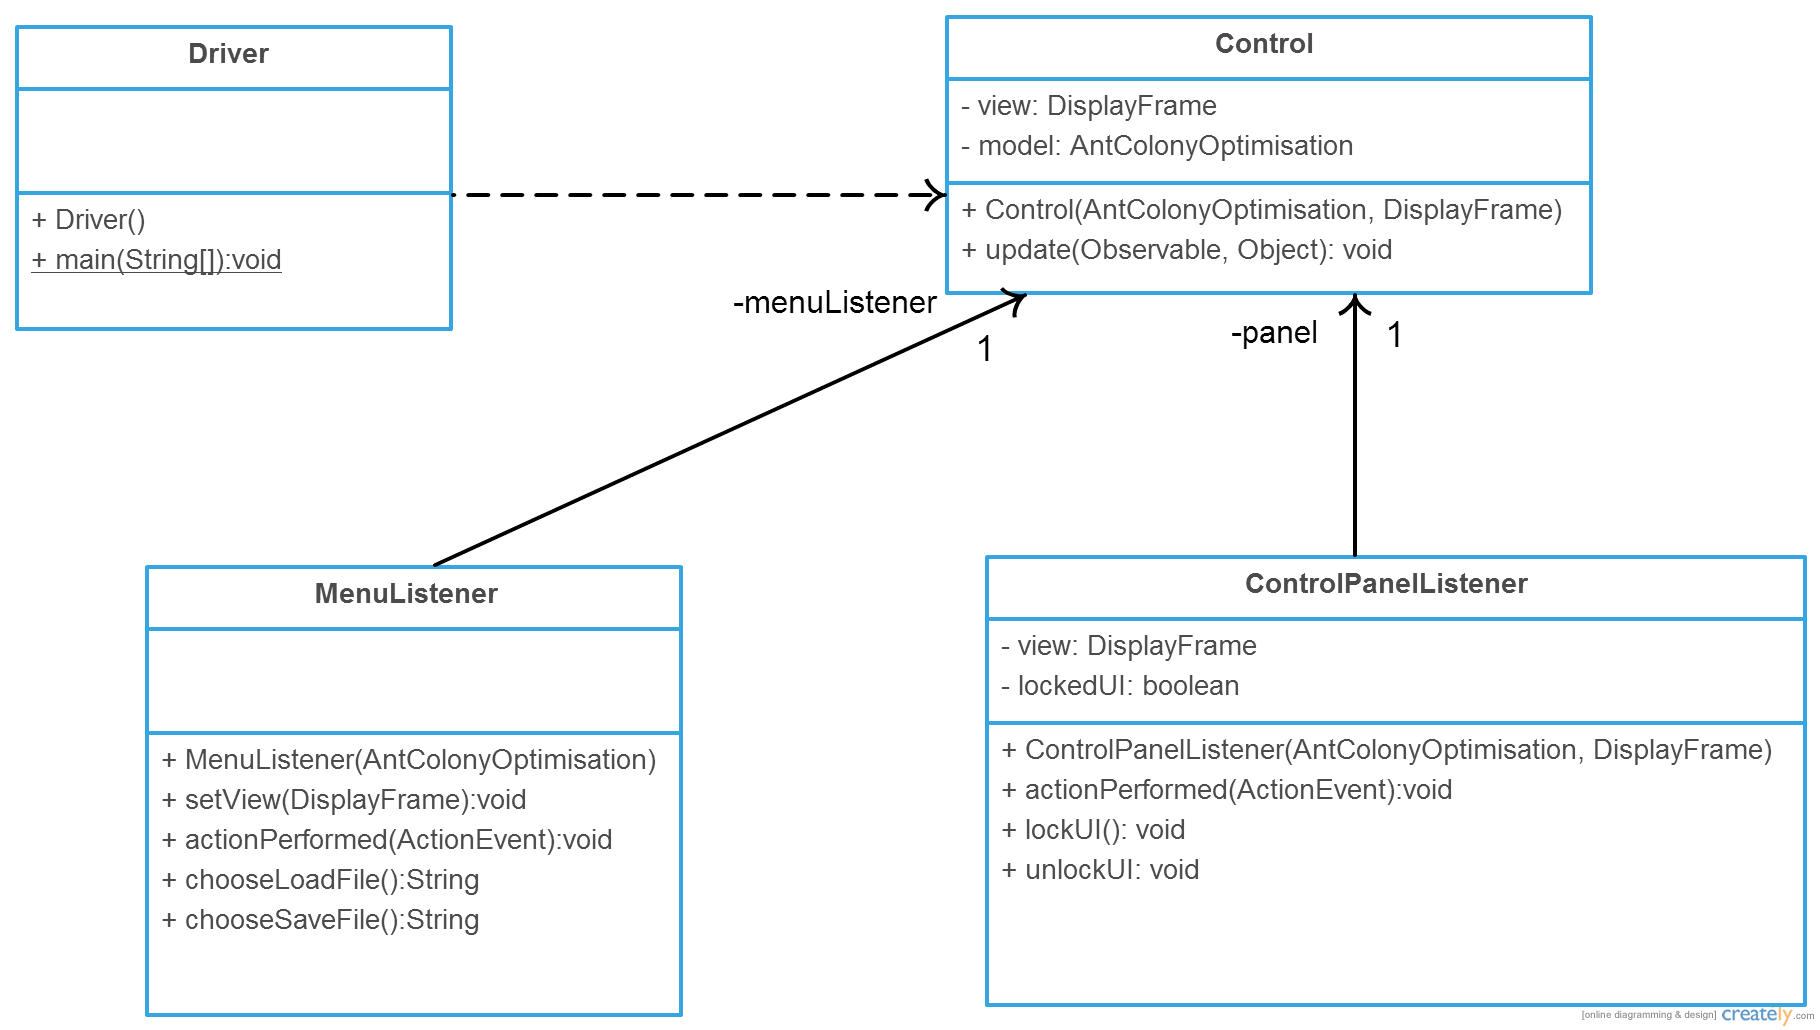
\includegraphics[scale=0.23]{Images/chapter4/controller}
\caption[Control Package Class Diagram]{The contents of the Controller package in standard UML Class diagram notation}
\label{fig:controllerImp}
\end{figure}

\subsubsection{Class Descriptions}

The Driver class remains largely unchanged from its initial proposed design (see appendix B, section \ref{driver:classdef}) however, it now interacts with the other components in a slightly different manner. The Driver class remains the sole entry point for the application. The Driver now has the additional responsibilities of instantiating the Control instance. The general purpose of the Driver class is still to ensure the system components are correctly instantiated, and holds no references to any instances of any object.

The Control as represented in figure \ref{fig:observableImp} is designed to observe the model and notify the view should the state of the model change significantly. In addition to this, the required instanced of MenuListener and ControlPanelListener are instantiated in this class and a reference to this Control object is maintained the created instances of said objects. The Control class is an additional feature not present in the initial design and is a result of the refactoring process. This class has the potential to be extended to support several other observable objects should this functionality be needed by the author in the future.

An instance of the MenuListener is used to listen the JMenuBar. This is designed collectively manage the actions represented by the elements contained in the JMenuBar. The alternative approach is to give each element in the JMenuBar its own Action Listener. This is far from efficient and increases both the codes complexity, and reduces overall maintainability of the application. The author decided to use a dedicated object such as this to listen to the menu and perform appropriate actions. This class maintains an instance of the Control class this enables the instance of this class to have access to the model and view instances stored in the Control instance enabling a simple way for the JMenuBar to have access to necessary functions.

A ControlPanelListener instance is designed to be a dedicated ActionListener for the ControlPanel (see section \ref{model:classdef}). Two separate ActionListeners are present in this application, this is because the author wanted to have dedicated listeners for each component, rather than having a combined object representing this class and the MenuListener. The author feels that this is appropriate as any modifications to the object which will be listened to becomes simpler to accomplish if relevant behaviours are extracted into logical modules such as this design exhibits.

\subsection{View}

The View package serves the same purpose as initial designed however, there has been a significant amount of refactoring applied to the initial design to enable a more effective graphical user interface to be created. The author has also added several new classes into this package to represent additional views which were not initially envisioned, but during development the author recognised that these new views were essential.

\clearpage
\begin{sidewaysfigure}
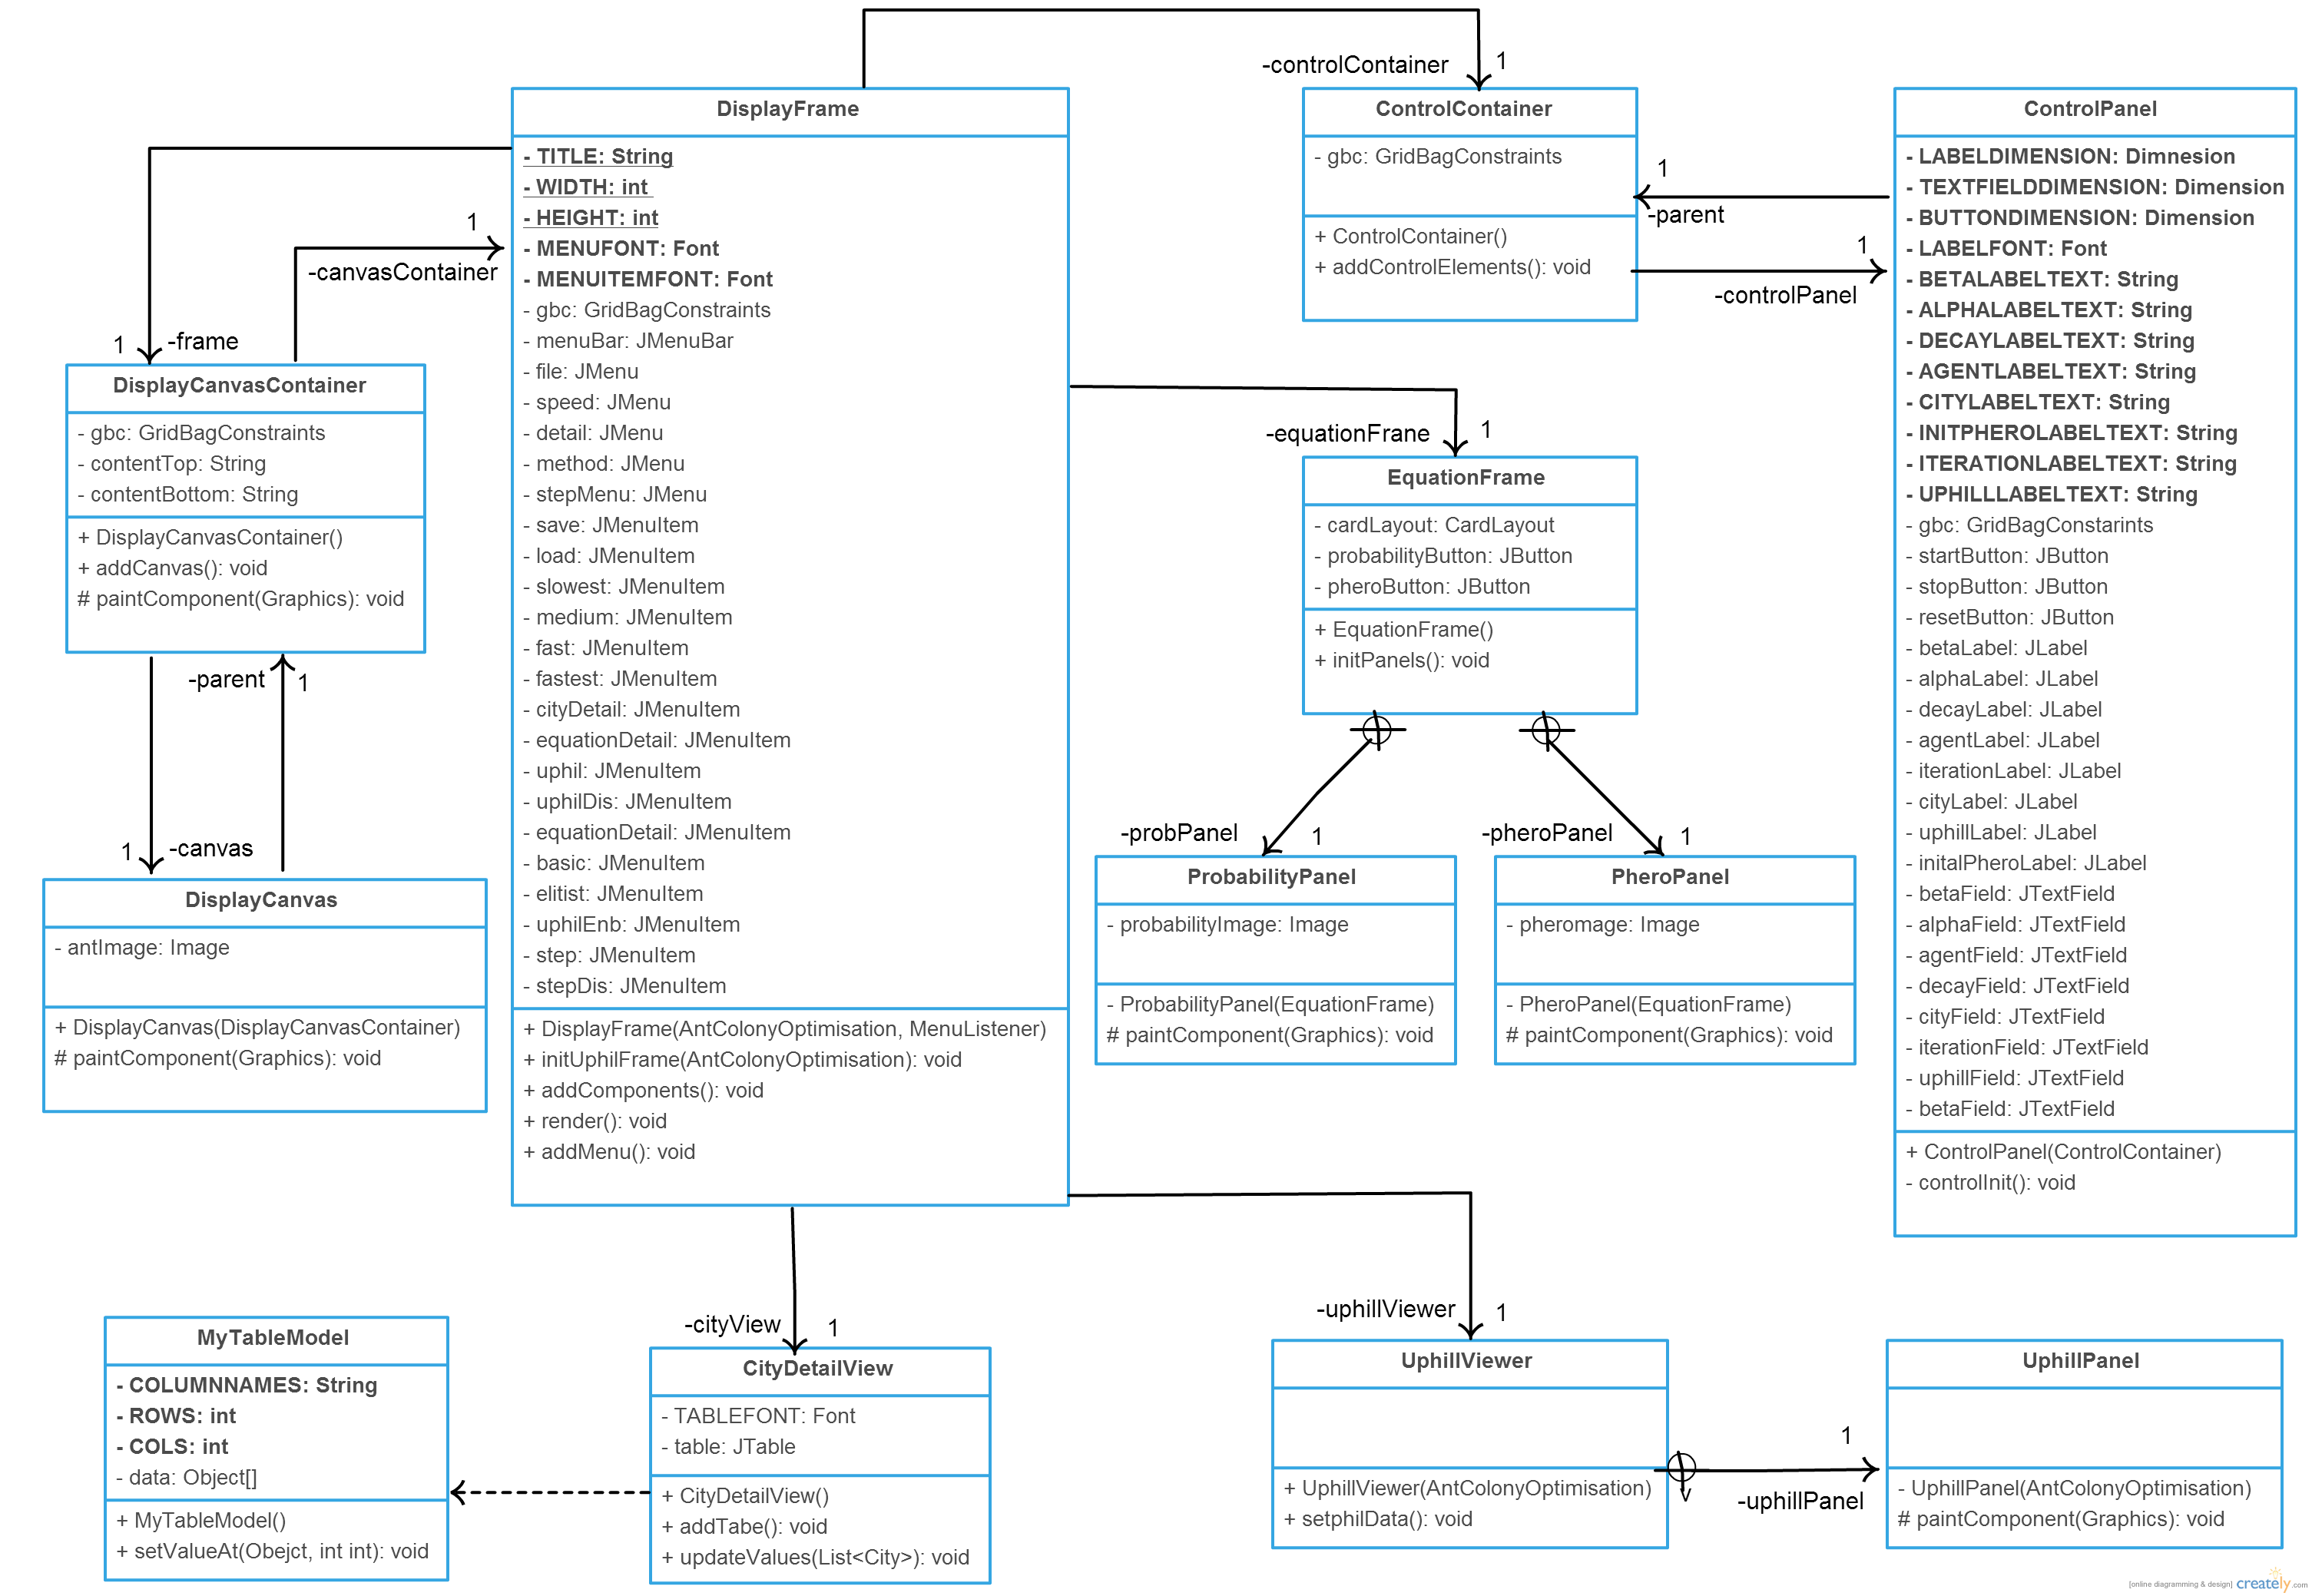
\includegraphics[scale=0.225]{Images/chapter4/view}
\caption[View Package Class Diagram]{The contents of the View package in standard UML Class diagram notation}
\label{fig:classdiagramImp}
\end{sidewaysfigure}
\clearpage

\subsubsection{Class Descriptions}
\label{view:clss}
Initially the DisplayFrame was designed to simply represent the highest level container which houses the remaining graphical user interface elements. As figure \ref{fig:classdiagram} shows the initial design for this class was very simplistic and lightweight. The author's decision to include additional user interface elements which were not originally planned has resulting in modification to the designed class. A JMenuBar has been added and as a result the DisplayFrame class grew in size in order to accommodate this JMenuBar and its necessary underlying elements. Although the size of this Class has grown the complexity and functionality is largely unchanged, it remains as the highest level container for the graphical user interface and control the instantiation of such elements.

The DisplayCanvasContainer is the result of renaming the DisplayPanel class in the initial design (figure \ref{fig:classdiagram}). This class is designed as a container to the DisplayCanvas instance, this functionality is as designed and the author has not modified its behaviour.

An instance of the DisplayCanvas class is used to visualise the algorithms state of execution to the users. This is the component that is painted during the algorithms execution using the $paintComponent$ method which it inherits from its JFrame super class. As the functionality provided by this Class is very simplistic, the current implementation remains unchanged from the initial design proposal (figure \ref{fig:classdiagram}).

The addition of the CityDetailView is a simple JFrame container which is used to display a JTable with data representing the number of agents currently at each city location. The JFrame displayed by this Class can be toggled between visible and invisible through user interaction with the respective JMenuBar item.

The structure of the table represented visually by the CityDetailView, is modelled by theMyTableModel class. Extracting the table’s structure into a separate class enables easy modification of the structure as well as reducing the coupling between the view and the table itself.

Similar to the DisplayCanvasContainer class, the ControlContainer is used to encapsulate the user input elements in their own separate container. This is a result of refactoring the UserInputPanel class in the initial design (figure \ref{fig:classdiagram}) into this container and the ControlPanel class. The main purpose for this class is to allow for a more diverse range of LayoutManagers to become available allowing for an easily modifiable interface.

The ControlPanel class used to contain the interface elements which directly relate to the creation and modification of the problem and world. This includes housing the text fields and labels required to enable the user to customise the algorithm parameters, as well as providing a simple means to start and stop the execution using a simple JButton approach. This class is essentially an extended version of the UserInputPanel class in the initial design (figure \ref{fig:classdiagram}) aside from the fact that more interface elements have been added the functionality is the same.

The EquationFrame class an extension of the JFrame Class which is used to display a graphic explaining the underlying algorithm functions. This class has no other functionality aside from the providing a means of displaying such graphics which is itself, contained within the ProbabilityPanel and PheroPanel Classes.

Both ProbabilityPanel and PheroPanel are nested classes inside the EquationFrame. These classes subclass JPanel and are used to contain different graphics which will be used to represent information relevant to the underlying probability and pheromone functions respectively.

The UphillViewer class is another new addition which was not perceived in the initial design. This class is a subclass of JFrame and is used to contain an UphillPanel instance. This JFrame can be togged between visible and invisible with relevant user interaction with the JMenuBar contained in the DisplayFrame.

An instance of the UphillPanel class is used to display information about the current status of the uphill routes for the current algorithms execution. This is an extension the JPanel class, enabling the uphill route data to be painted to the component using the inherited $paintComponent$ method. This is a nested class inside UphillView as no other objects uses or needs the knowledge of this a nested class is the most suitable way to contain it.

\subsection{Model}

The elements contained in the initial proposed designed represented in figure \ref{fig:classdiagram} has undergone significant refactoring which has produced a vastly different structure. During the development process the author found the the initial design happened to be inadequate for representing the algorithm in a suitable manner as it lacked necessary components and detail.

\clearpage
\begin{sidewaysfigure}
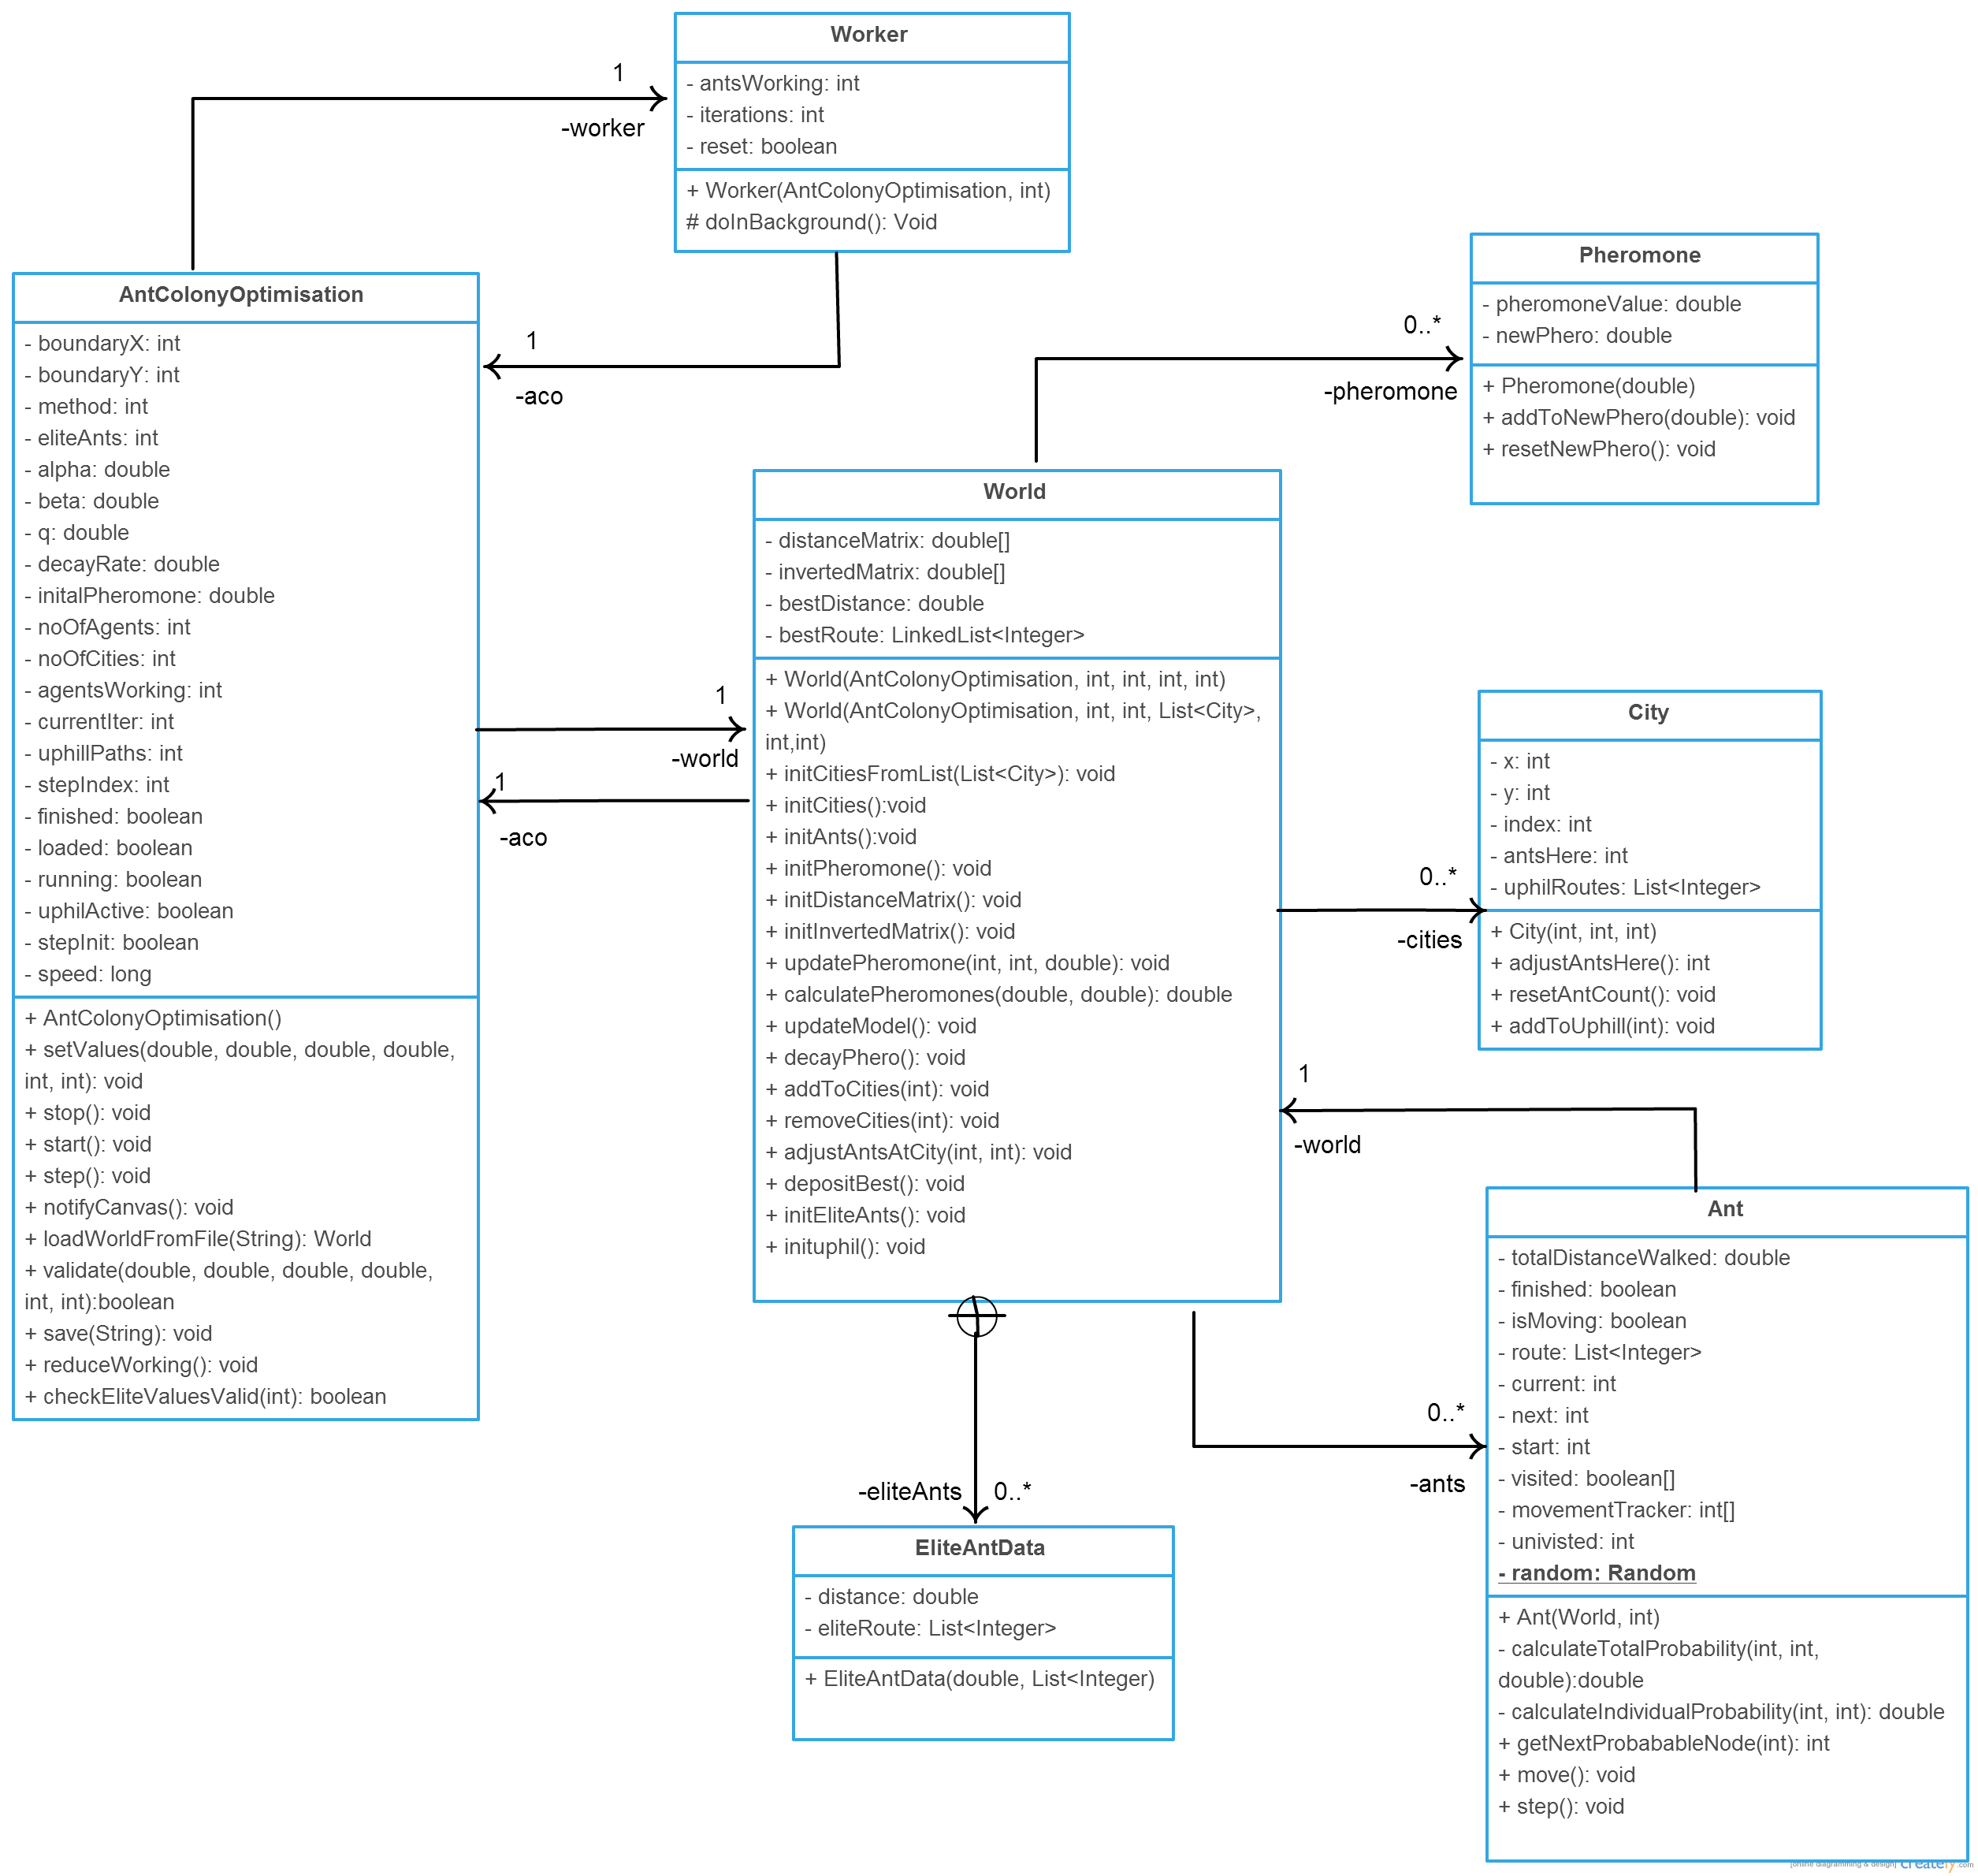
\includegraphics[scale=0.22]{Images/chapter4/model}
\caption[Model Package Class Diagram]{The contents of the Model package in standard UML Class diagram notation}
\label{fig:classdiagramImp}
\end{sidewaysfigure}
\clearpage

\subsubsection{Class Descriptions}
\label{model:classdef}

The initial concept behind the AntColonyOptimisation class is that this serves as the main control point and data centre for the algorithms execution. This class is used to store all the necessary parameter values and is also responsible for the instantiation of the Word representation. This class also controls external package access to the Model package and its data. This largely remains the same as designed however, there are slight modifications to accommodate additional functionality.

The Worker class was something that wasn’t initially planned. As discussed in \ref{swingmeupm8} there was a necessity for a way to control the algorithms execution without interfering with the performance of the interface. This class is an extension of the SwingWorker class and uses the inherited $doInBackground$ method to perform the algorithms execution in a suitable manner. 

The World class is used to model the problem representation and the environment for which the agents will be deployed during the algorithms execution. This class houses all the data relevant to such representations including a List of all Ant and City objects as well as having basic data structures which provide an effective representation of the pheromone concentrations for every edge within the graph and controls the manipulation of pheromones on such edges. This class is generally the same as proposed in figure \ref{fig:classdiagram} however slight modifications have been made to support additional features.

A City object is used to represent a node in the current problem representation graph. A collection of these City objects is maintained in the current World instance, and iterated through during both the solving and painting processes.

A Pheromone object is used to model the pheromone concentrations for any given edge. A two-dimensional array of these Objects is maintained in the current World instance, and these Objects are constantly manipulated during the pheromone deposit and decay operations. 

An Ant object is used to represent an agent which will be deployed in the current environment in order to solve the current problem. The World instance will maintain a collection of these objects. Each Ant has sufficient variables and methods to enable them to move and deposit pheromones accordingly. The initial design suggested the use of an AntInterface, however as the author has decided that there will only be one type of Ant thus, the interface is deemed to be unnecessary. Generally, this class is as designed in Figure \ref{fig:classdiagram}.

The EliteAntData is a nested class inside the World which is used to store the current elite routes. This feature is only necessary if the user has selected the Elitist Ant System as the current algorithm type. This is required to correctly preserver the best routes across iterations as the ant objects get reset each iteration. Rather than storing a whole ant object the author has opted only to store the best distances and best routes as this has less overheads when compared to storing an ant in full.

\subsection{Utils}

During development the noticed that some methods were being implemented in numerous locations. To prevent code duplication and promote re-usability the Utils package was implemented. This is a very simple package, containing one class however, the contents of this class don't belong in any other package individually.

\begin{figure}[H]
\centering
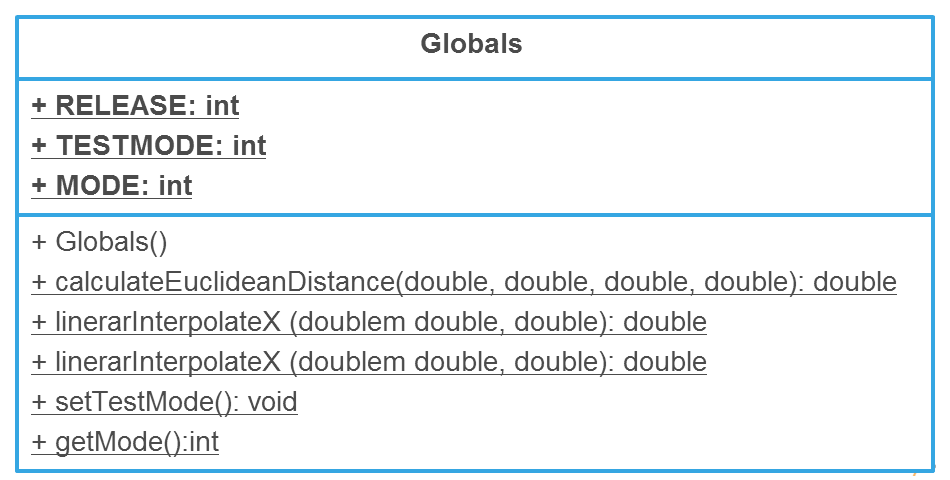
\includegraphics[scale=0.3]{Images/chapter4/gloabls}
\caption[Utils Package Class Diagram]{The contents of the Utils package in standard UML Class diagram notation}
\label{fig:utilsImp}
\end{figure}

Figure \ref{fig:utilsImp} represents the single class contents of the Utils package. This Globals class contains several publicly available static variables and methods enabling application wide access. This enables the multiple packages which rely on the results of such methods to retain access to them whilst also reducing the amount of repeated code. In addition this class enables the execution mode to be switched from release to test mode. When in test mode the error messages require no user response enabling the automated test process to complete more easily.

\subsection{System Interactions}

The different packages and their contents have been described above however, the interactions between packages must be carefully designed to ensure correct implementation and of the Model-View-Controller design pattern. 

\clearpage
\begin{sidewaysfigure}
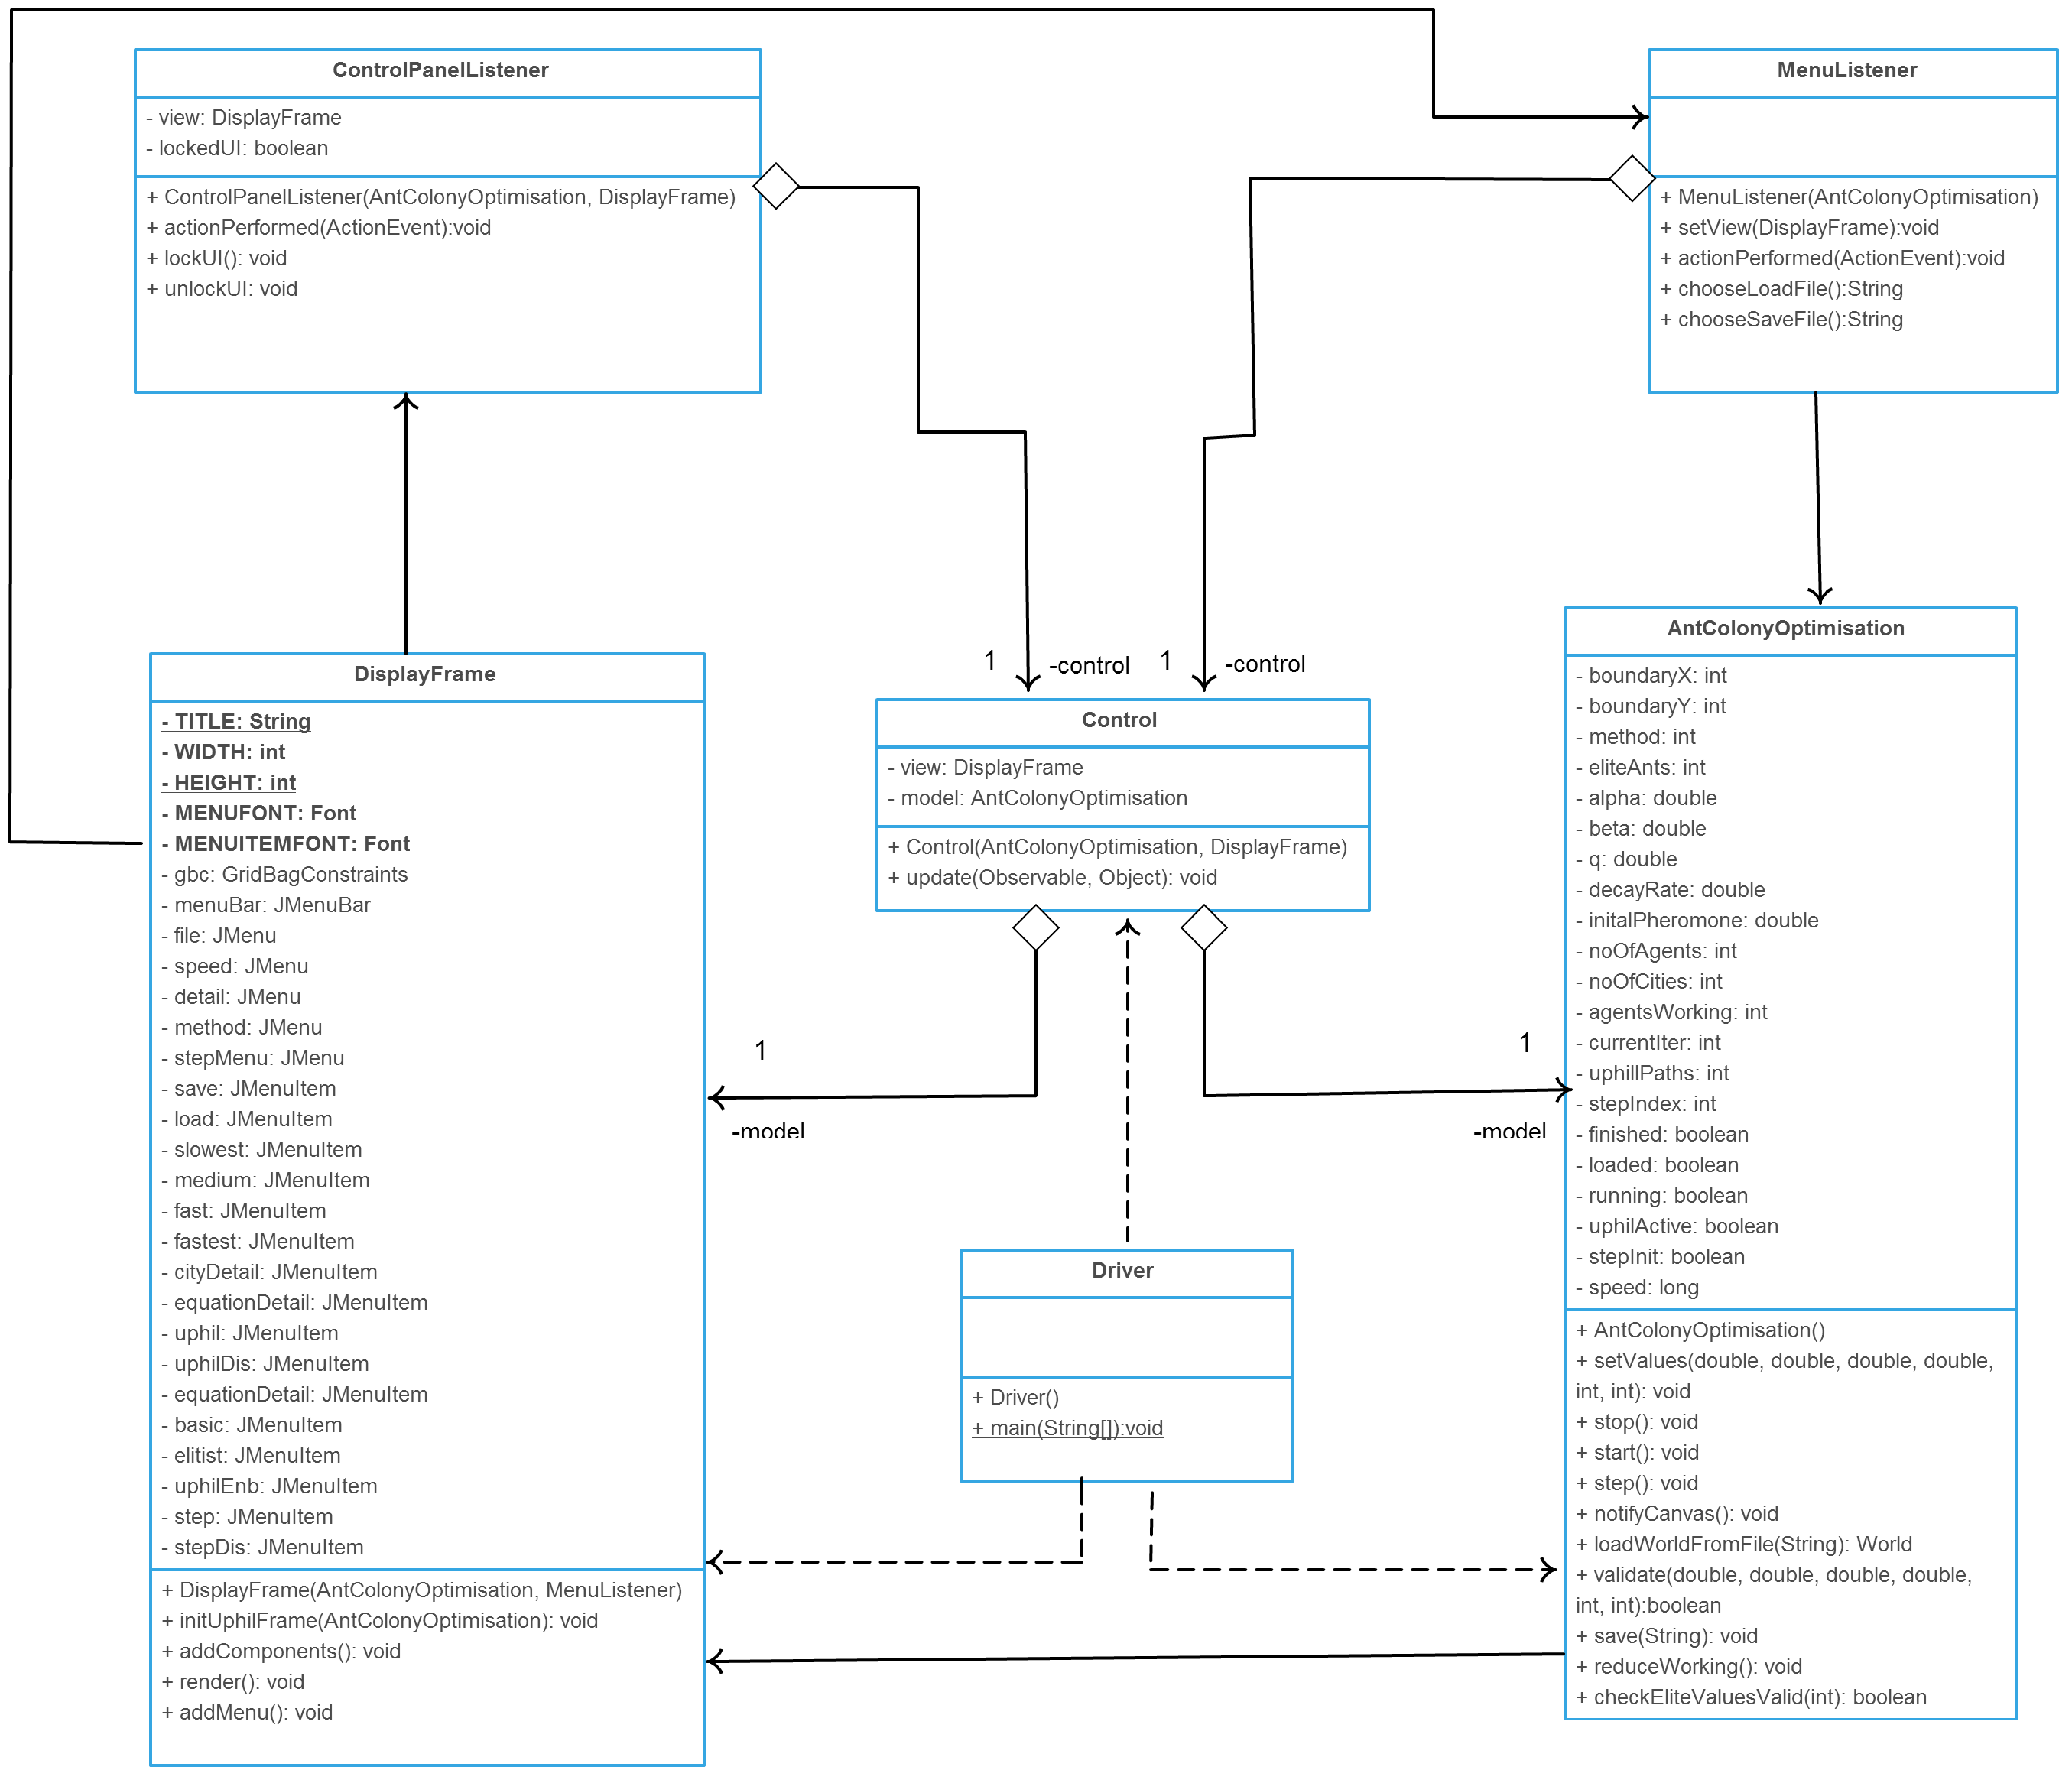
\includegraphics[scale=0.22]{Images/chapter4/overallClassinteraction}
\caption[Package Interaction Diagram]{The proposed manner of package interaction expressed in standard UML Class diagram notation.}
\label{fig:interacttion}
\end{sidewaysfigure}
\clearpage

Figure \ref{fig:interacttion} demonstrates how the access to the View and Model packages is governed by the instances of the DisplayFrame and AntConolonyOptimisation respectively. This keeps the interaction between packages simple and enables encapsulation of sensitive data. This design adheres to the Model-View-Controller principles as the Controller package and its contents govern the interactions between the Model and View. The view, has no reference to the model however, at runtime an instance of the AntConolonyOptimisation is passed to the View in order for the painting of necessary components to take place. As there is no explicit link between the model and view these packages can be easily modified or substituted in order to change the current representation there is no coupling between the contents of these packages.

\section{Design Patterns}
\subsection{Model-View-Controller}
The current design still adheres to the Model-View-Controller(MVC) principles discussed in Appendix B, section \ref{sssec:mvc} however, the complexity of the different package elements has increased. As designed, the author has implemented an MVC compliant architecture through the use of the Observer and Observable relationship using the corresponding default Java framework. The general concept is implemented as defined in appendix B, section \ref{obby} slight modifications have been made to the classes representing the different components of the Observer and Observable concept.

\begin{figure}[H]
\centering
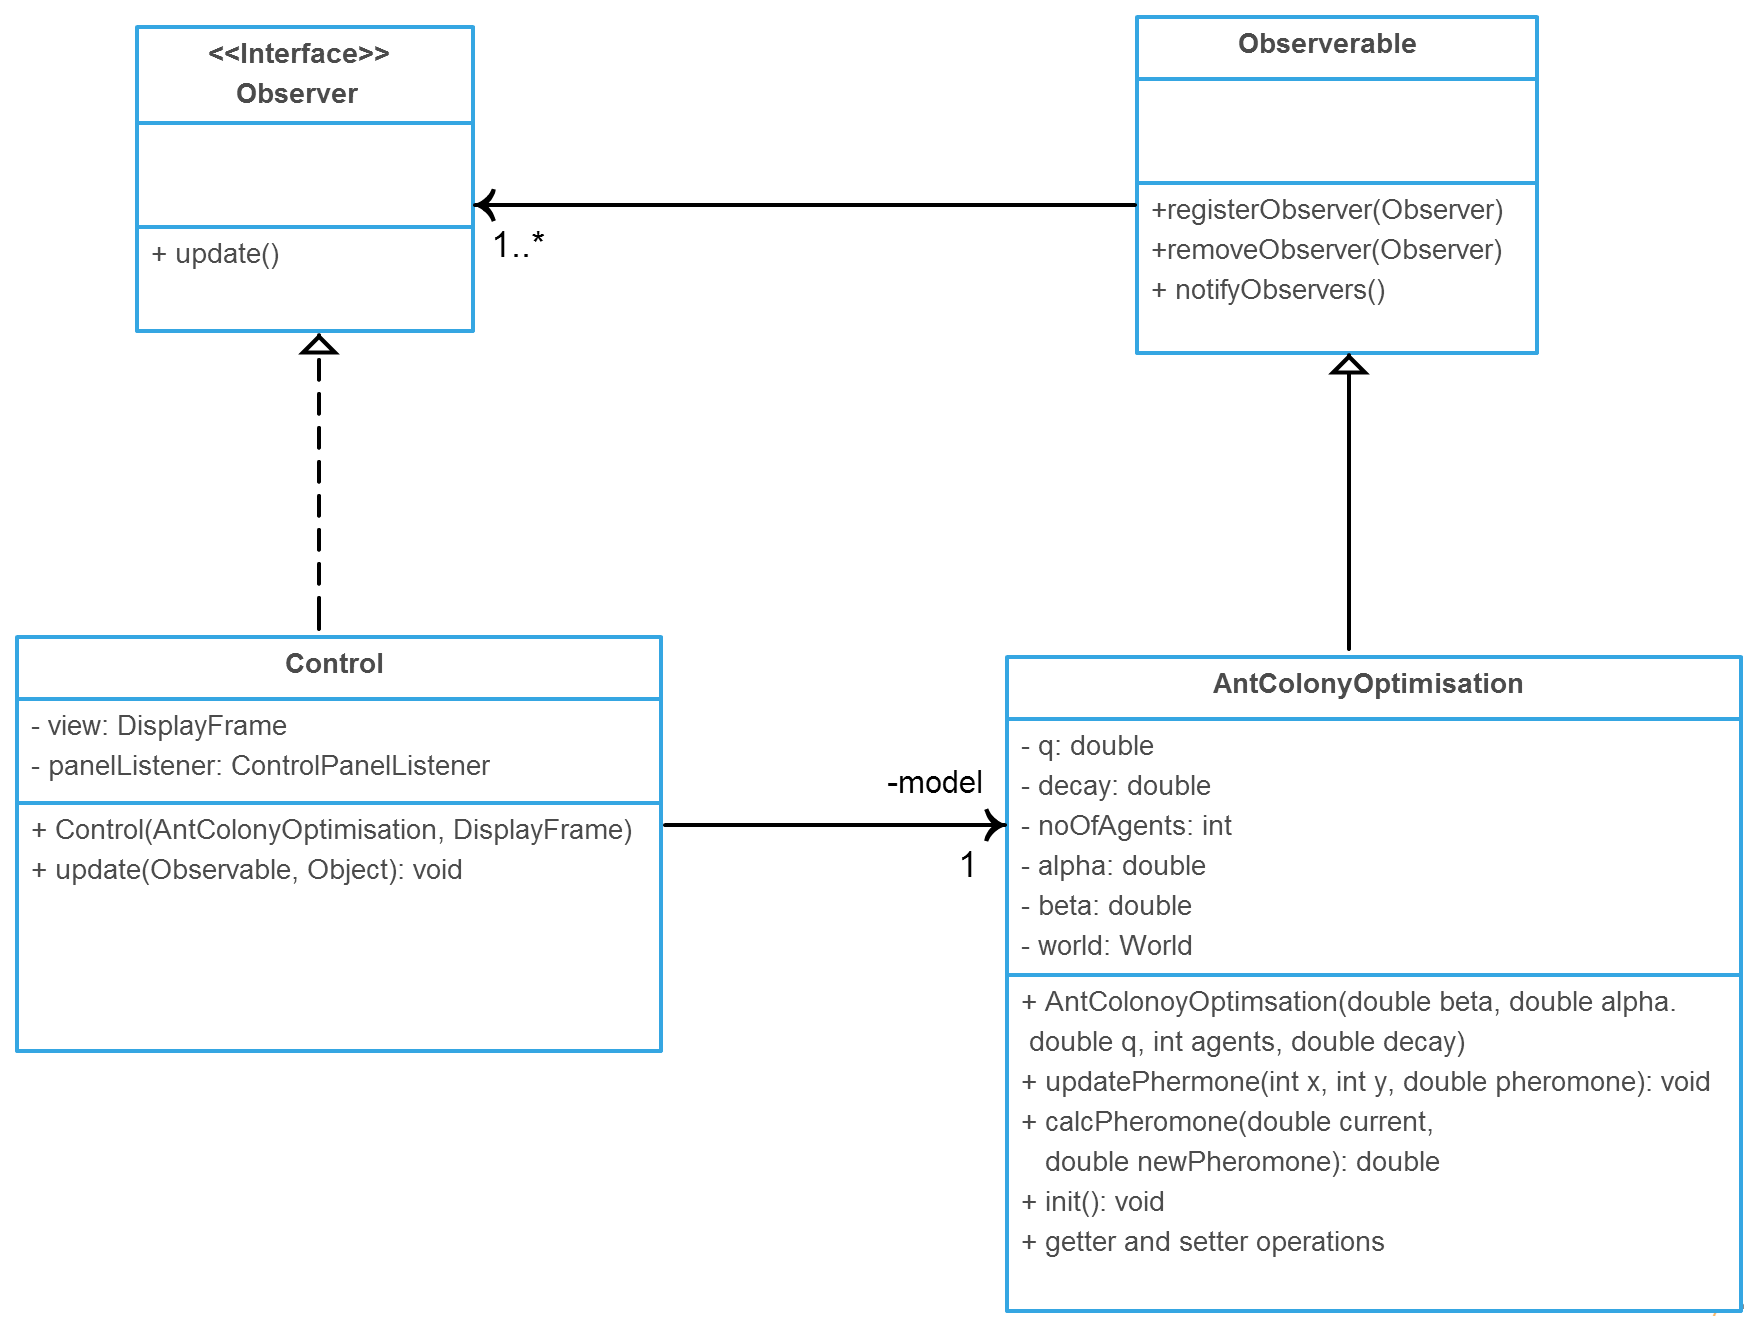
\includegraphics[width=0.9\textwidth]{Images/chapter4/observerImplemetation}
\caption[Observer and Observable Implementation]{Implementation of the Observer and Observable Design pattern}
\label{fig:observableImp}
\end{figure}

Figure \ref{fig:observableImp} demonstrates how the Control class will implement the Observer interface. This listens to the Observable object and determines the correct actions based upon the source of update. The AntColonyOptimisation class is as defined in section \ref{model:classdef} and acts as the observable object through its extension of the Observable super class. This inheritance grants the AntColonyOptimisation instance access to key methods such as $registerObserver()$ this allows the author to assign the Control instance as the designated observer. The $notifyOberservers()$ methods enables the author to dictate when updates are published to the Control instance which will the correctly update the View.

\subsection{Singleton}

Initially the author proposed that classes that compose the user interface would implement the Singleton design pattern\cite{gof:design:singleton}, an example this proposed design can be seen in appendix B, section \ref{sssec:singleton}. The author had initially implemented the interface witch each class implementing the Singleton pattern which caused complications. The Singleton pattern is however absent in the current architecture. As the instance of a Singleton object is globally accessible, difficulties arose during the application debugging. This issue happened to be more prevalent when extending the functionality provided by each of the Singleton classes, for example the DisplayFrame class now contains a wider range of functionality than initial planned. Not only did the Singleton instance complicate the addition of these extended features, debugging these features became more difficult as the global accessibility made it harder to track the source of the bug itself. This is due the fact that it is easy to accidently interact and modify a global variable or instance. Often the source of these bugs was not where the author expected and were often due to an incorrect interactions with these new extensions in a separate package. This was the main reason the author decided to withdraw the use of the Singleton pattern as the author felt it was much simpler to not have global access to these instances and features.

Robert Martin propositioned idea of the Single Responsibility Principle (SRP) in 1990 \cite{SRP:site}. The general concept behind the SRP is that each logical module in the software should have one reason to change or model one specific responsibility rather than a collection of unrelated features or functions. If a module has been extended to support multiple unrelated features, the SRP states that the unrelated features should be extracted into relevant modules so that each module maintains its one responsibility. The author feels that implementing the Singleton in the proposed manner (see appendix B, section \ref{sssec:singleton}) violated the underlying concepts of the SRP. As the Singleton class is responsible for tracking and instantiation of its one allowed instance and the functionality which the module presents, this class now has more than one responsibility and thus violates the SRP. The author believes the SRP should be regarded highly during development in order to produce maintainable and extendable software. As a result he has opted for adhering to the SRP over the Singleton implementations. The author experimented with the idea of having extracting the functionality of the Singleton classes and the tracking of the instance of such classes into separate system modules however, this vastly overcomplicated the architecture.

Overall, the author sees the implementation of the Singleton Design pattern as more of an anti-pattern. As this is the case and to enable easier modification the implementation of any Singleton class as initially designed has been removed. Solutions the above problems could be refactored in, but this is seen as unnecessary complexity by the author and has therefore also been omitted.

\section{User Interface}
\label{interfacebrah}
The user interface elements will be designed with the three laws of user interaction discussed in section \ref{uiMethods} as a top priority. The interfaces will be consistent in theme and styling which will provide application wide consistency for the user.

\subsection{Main Display}

The design for the main display, which refers the general view the user will be presented and interact with remains unchanged from the initial proposal as represented in figure \ref{fig:interface}. There has been modifications to this design during the implementation phase however, these the authors flexible process (see section \ref{processSec}) and the fact that these changes were fairly trivial allowed the author to implement them without any prior design, section \ref{mainimp} displays the implemention of this design and said changes.

\subsection{UphillViewer}
\label{uphillview}

The uphill viewer was not an element of the user interface which was initially planned, however the addition to implement the ability for a path to represent uphill terrain required a view to summarize which of these paths are in fact subject to this uphill modification. This interface is a result of the contents of the UphillViewer class (see section \ref{view:clss}).

\begin{figure}[H]
\centering
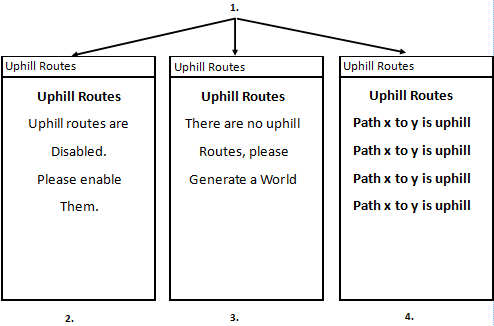
\includegraphics[scale=0.7]{Images/chapter4/uphilviews}
\caption[UphillViewer Design]{Proposal for the UphillViewer interface representing the different states possible at runtime.}
\label{fig:uphillViewImp}
\end{figure}

\textbf{1.} in figure \ref{fig:uphillViewImp} is used to demonstrate each possible state for the UphillViewer contained in the same high level container. \textbf{2.} is used to show the default state and content for the UphillViewer interface. This state is shown to the user if uphill route generation is currently disabled, and prompts the user to enable them. \textbf{3.} is shown to the user if uphill routes generation is enabled, but the current world is yet to be generated. \textbf{4.} is shown to the user when both uphill route generation is enabled and such routes have been generated. The $x$ and $y$ values in this figure will be replaced with indexes of valid cities to enable to the user to understand which routes are deemed uphill.

%4943 WORDS AS OF THIS POINT
\subsection{CityDetail View}
\label{deetzlview}

The CityDetailView is used to summarize how many agents are currently at each City. This view was not initially designed however, the author felt that this was a necessary addition and therefore designed a rough outline of such interface.

\begin{figure}[H]
\centering
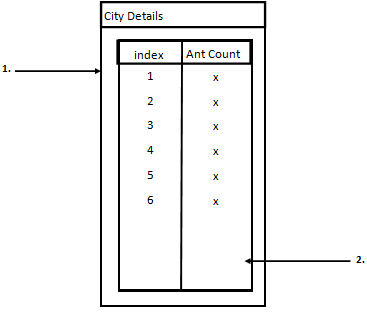
\includegraphics[scale=0.7]{Images/chapter4/citydetails}
\caption[CityDetailViewer Design]{Proposal for the CityDetailViewer interface.}
\label{fig:deetzViewImp}
\end{figure}

\textbf{1.} in figure \ref{fig:deetzViewImp} represents how this view is contained in a separate container to the main display. This enables the user to move this view around as desired in order to customise the current view to their liking. \textbf{2.} demonstrates how the contents of the CityDetailView will be displayed (see section \ref{view:clss}). The number of rows will directly relate to the number of City objects in the current collection. The $x$ values will be substituted for the correct number of ants at the corresponding city index.

\subsection{EquationFrame}
\label{eqnlview}

The Equation Viewer is used to explain the functions that the underlying algorithm uses. This view was not initially designed however, the author felt that this was a necessary addition and therefore designed a rough outline of such interface.

\begin{figure}[H]
\centering
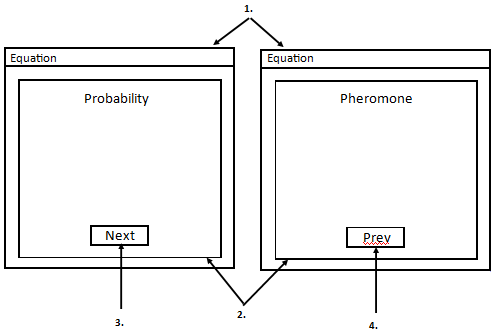
\includegraphics[scale=0.7]{Images/chapter4/pheroprobpanels}
\caption[EquationFrame Design]{Proposal for the EquationFrame interface.}
\label{fig:eqnViewImp}
\end{figure}

\textbf{1.} in figure \ref{fig:eqnViewImp} represents how this view is contained in a separate container to the main display. This enables the user to move this view around as desired in order to customise the current view to their tastes. \textbf{2.} demonstrates how there will one shared panel which will be used to display the content related to both the pheromone and probability equations. The content of the container signified by \textbf{2.} will be substituted for the correct content when the user interacts with either one of the buttons signified by \textbf{3.} and \textbf{4.}. If the user interacts with the button \textbf{3.} then the content of the container will switch and will now represent details about the pheromone equation. When button \textbf{4.} is pressed by the user, the content of the container will now reflect the information stored about the probability equation. The author has designed this such that any additional equations can be implemented in the same way using simple button navigation without the need of significant extensions to the existing framework.

\subsection{Error Feedback}
The interfaces responsible for error feedback have been carefully designed so that the author can effectively inform the user of the error, the cause of the error, and solution of such error. These interfaces are designed to be abstract in such a manner so the same interface can be used to represent several different related error responses.

\subsubsection{Parameter Errors}
\label{paramerror}
These errors are produced when a user has defined a value for an algorithm parameter which is deemed to be illegal. This illegal value could mean that the value the user has entered is outside of the scope of accepted value or the user has specified an illegal type for this parameter. An illegal type a situation such as entering a double value where an integer is required.

The design for these error messages remains as shown in section \ref{error:proposal}, appendix B. This design is simple and effective and provides the user with everything they need to know about the errors source and solution. This interface can be re used for any parameter related error as the only modification would be the change of the interfaces content, there would be no need to implement or design a new interface.

\subsubsection{File IO Errors}

The ability for a user to load or save a problem configuration to a selected file is a new addition to the system. The design of these error interfaces is based off of the design for the parameter error interfaces described in section \ref{paramerror}. 

\begin{figure}[H]
\centering
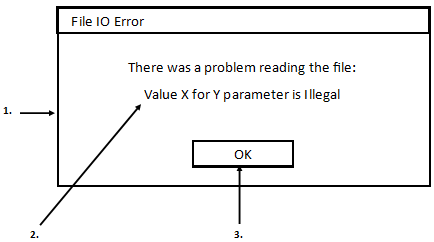
\includegraphics[scale=0.7]{Images/chapter4/IOError}
\caption[File IO Error Feedback Design]{Design of the File IO error feedback interface.}
\label{fig:ioErrors}
\end{figure}

Similar to the parameter error interface, this interface as described in figure \ref{fig:ioErrors} will provide the user with concise feedback as to how and why the file IO process did not complete as expected. From the error message displayed the user should be able to deduce their own solution to the problem. As there are numerous problems which could arise with file IO, the author decided to omit providing a solution to the user. Instead the erroneous data is flagged to the user enabling them to locate the problem and resolve it. The $x$ value in figure \ref{fig:ioErrors} will be replaced with the problematic value whereas the $y$ value will refer to the problematic parameter.

\section{Algorithms}

This section covers the abstract implementation of the key algorithms used for both modelling the algorithms execution and the visualisation of such process.

\subsection{General Overview}

The general algorithm remains largely unchanged from the initially proposed algorithm in section \ref{algym8}, appendix B. The author has amended this design slightly to factor in the change of problem representation. As the TSP is the default problem representation the initial ideas behind ants collecting food and returning to the nest have been replaced by conditionals reflecting if an agent has visited every City or not.

\begin{algorithm}[H]
\caption[Ant System Pseudo-code]{Pseudo-code for Ant System implementation}
\label{aco:pseudo2}
\begin{algorithmic}[1]
\State Initialise AntColonyOptimisation with defined parameters
\If{$!parameters\ are\ legal$}
\State Display error message to user
\State $return$
\EndIf 
\State \textbf{end if}
\State Initialise World with algorithm parameters
\State Initialise $Nodes$ and graph
\State Initialise \textit{pheromone} values
\State Initialise $Agents$
\While {$!all\ agents\ finished$} 
\ForAll{Agents}
\While{!visited\ all\ $City$\ locations}
\State Calculate next move using probabilistic function 
\State Add location to Agent's memory
\State update pheromone
\State Update the View
\EndWhile 
\State \textbf{end while}
\EndFor 
\State \textbf{end for}
\EndWhile
\If{$\textit{local best solution} < \textit{global best solution}$}
\State $global best = local\ best\ solution$
\EndIf
\State \textbf{end if}
\State \textbf{end while}
\State output \textbf{global best} solution
\end{algorithmic}
\end{algorithm}
%5854 words up to this point

This pseudo code remains largely unchanged from the initial design represented by algorithm \ref{aco:pseudo}, appendix B. There has been the modification of the conditional statement represented by line 12 in algorithm \ref{aco:pseudo2}. This change reflects the updated problem representation so that agents now visit all City locations rather than focussing on a nest and food situation.

\begin{sidewaysfigure}
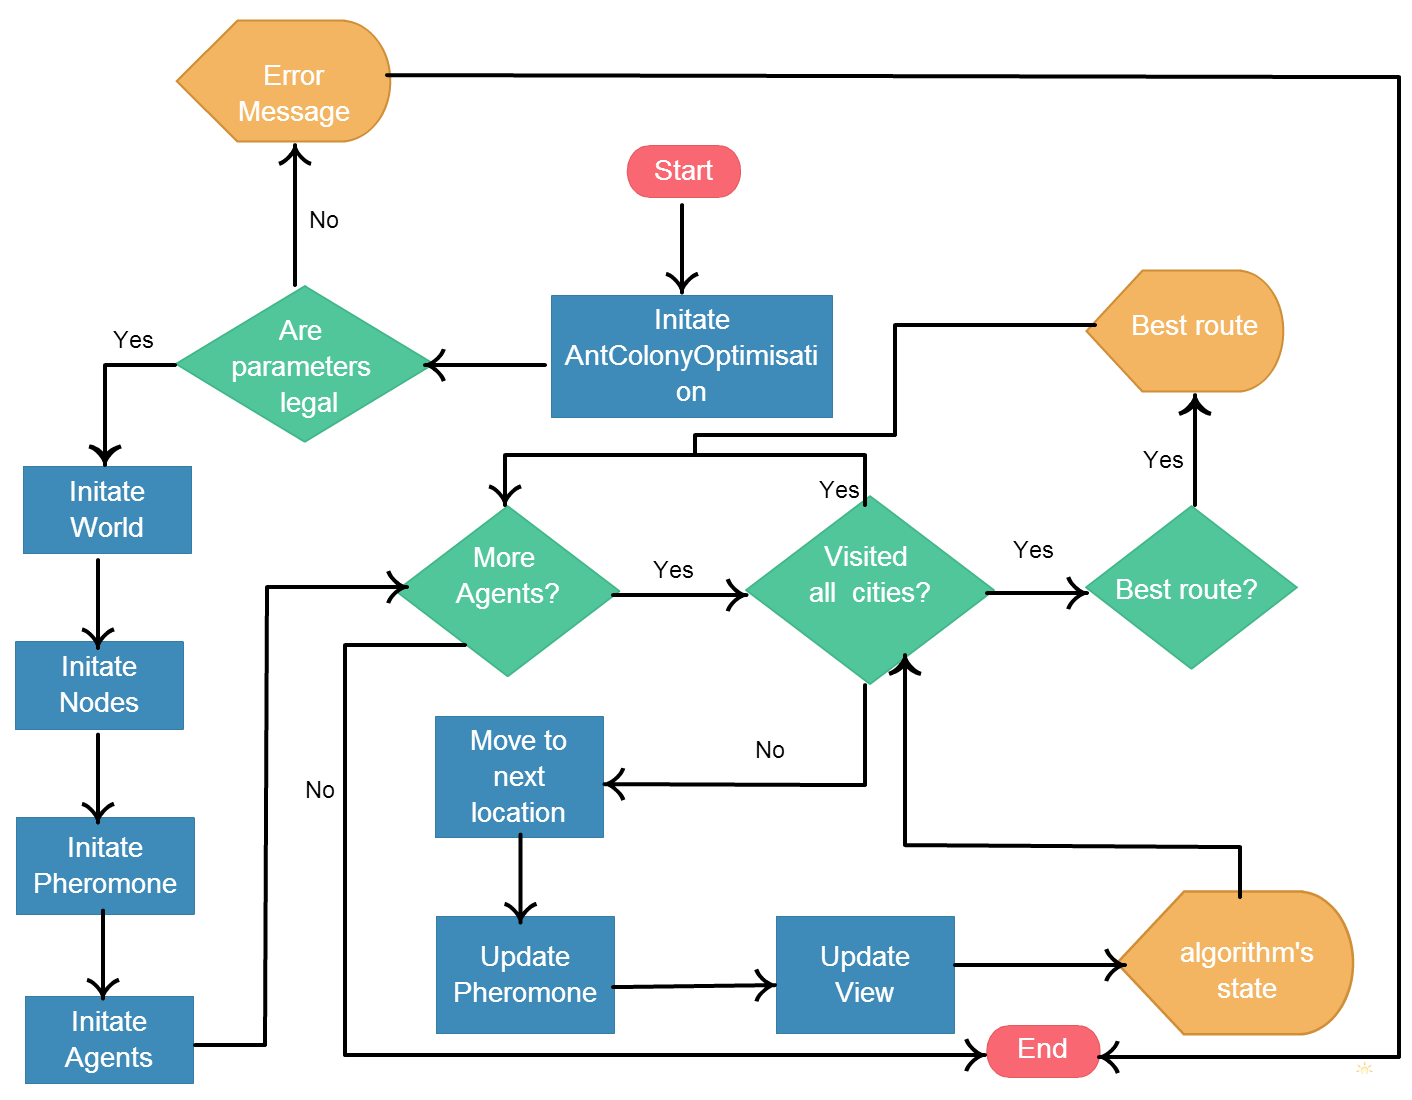
\includegraphics[scale=0.45]{Images/chapter4/overallflow}
\caption[Basic Ant System Flow Diagram]{Flow diagram representing the algorithm described in algorithm \ref{aco:pseudo2}}
\label{fig:overallFlow}
\end{sidewaysfigure}

\begin{figure}[H]
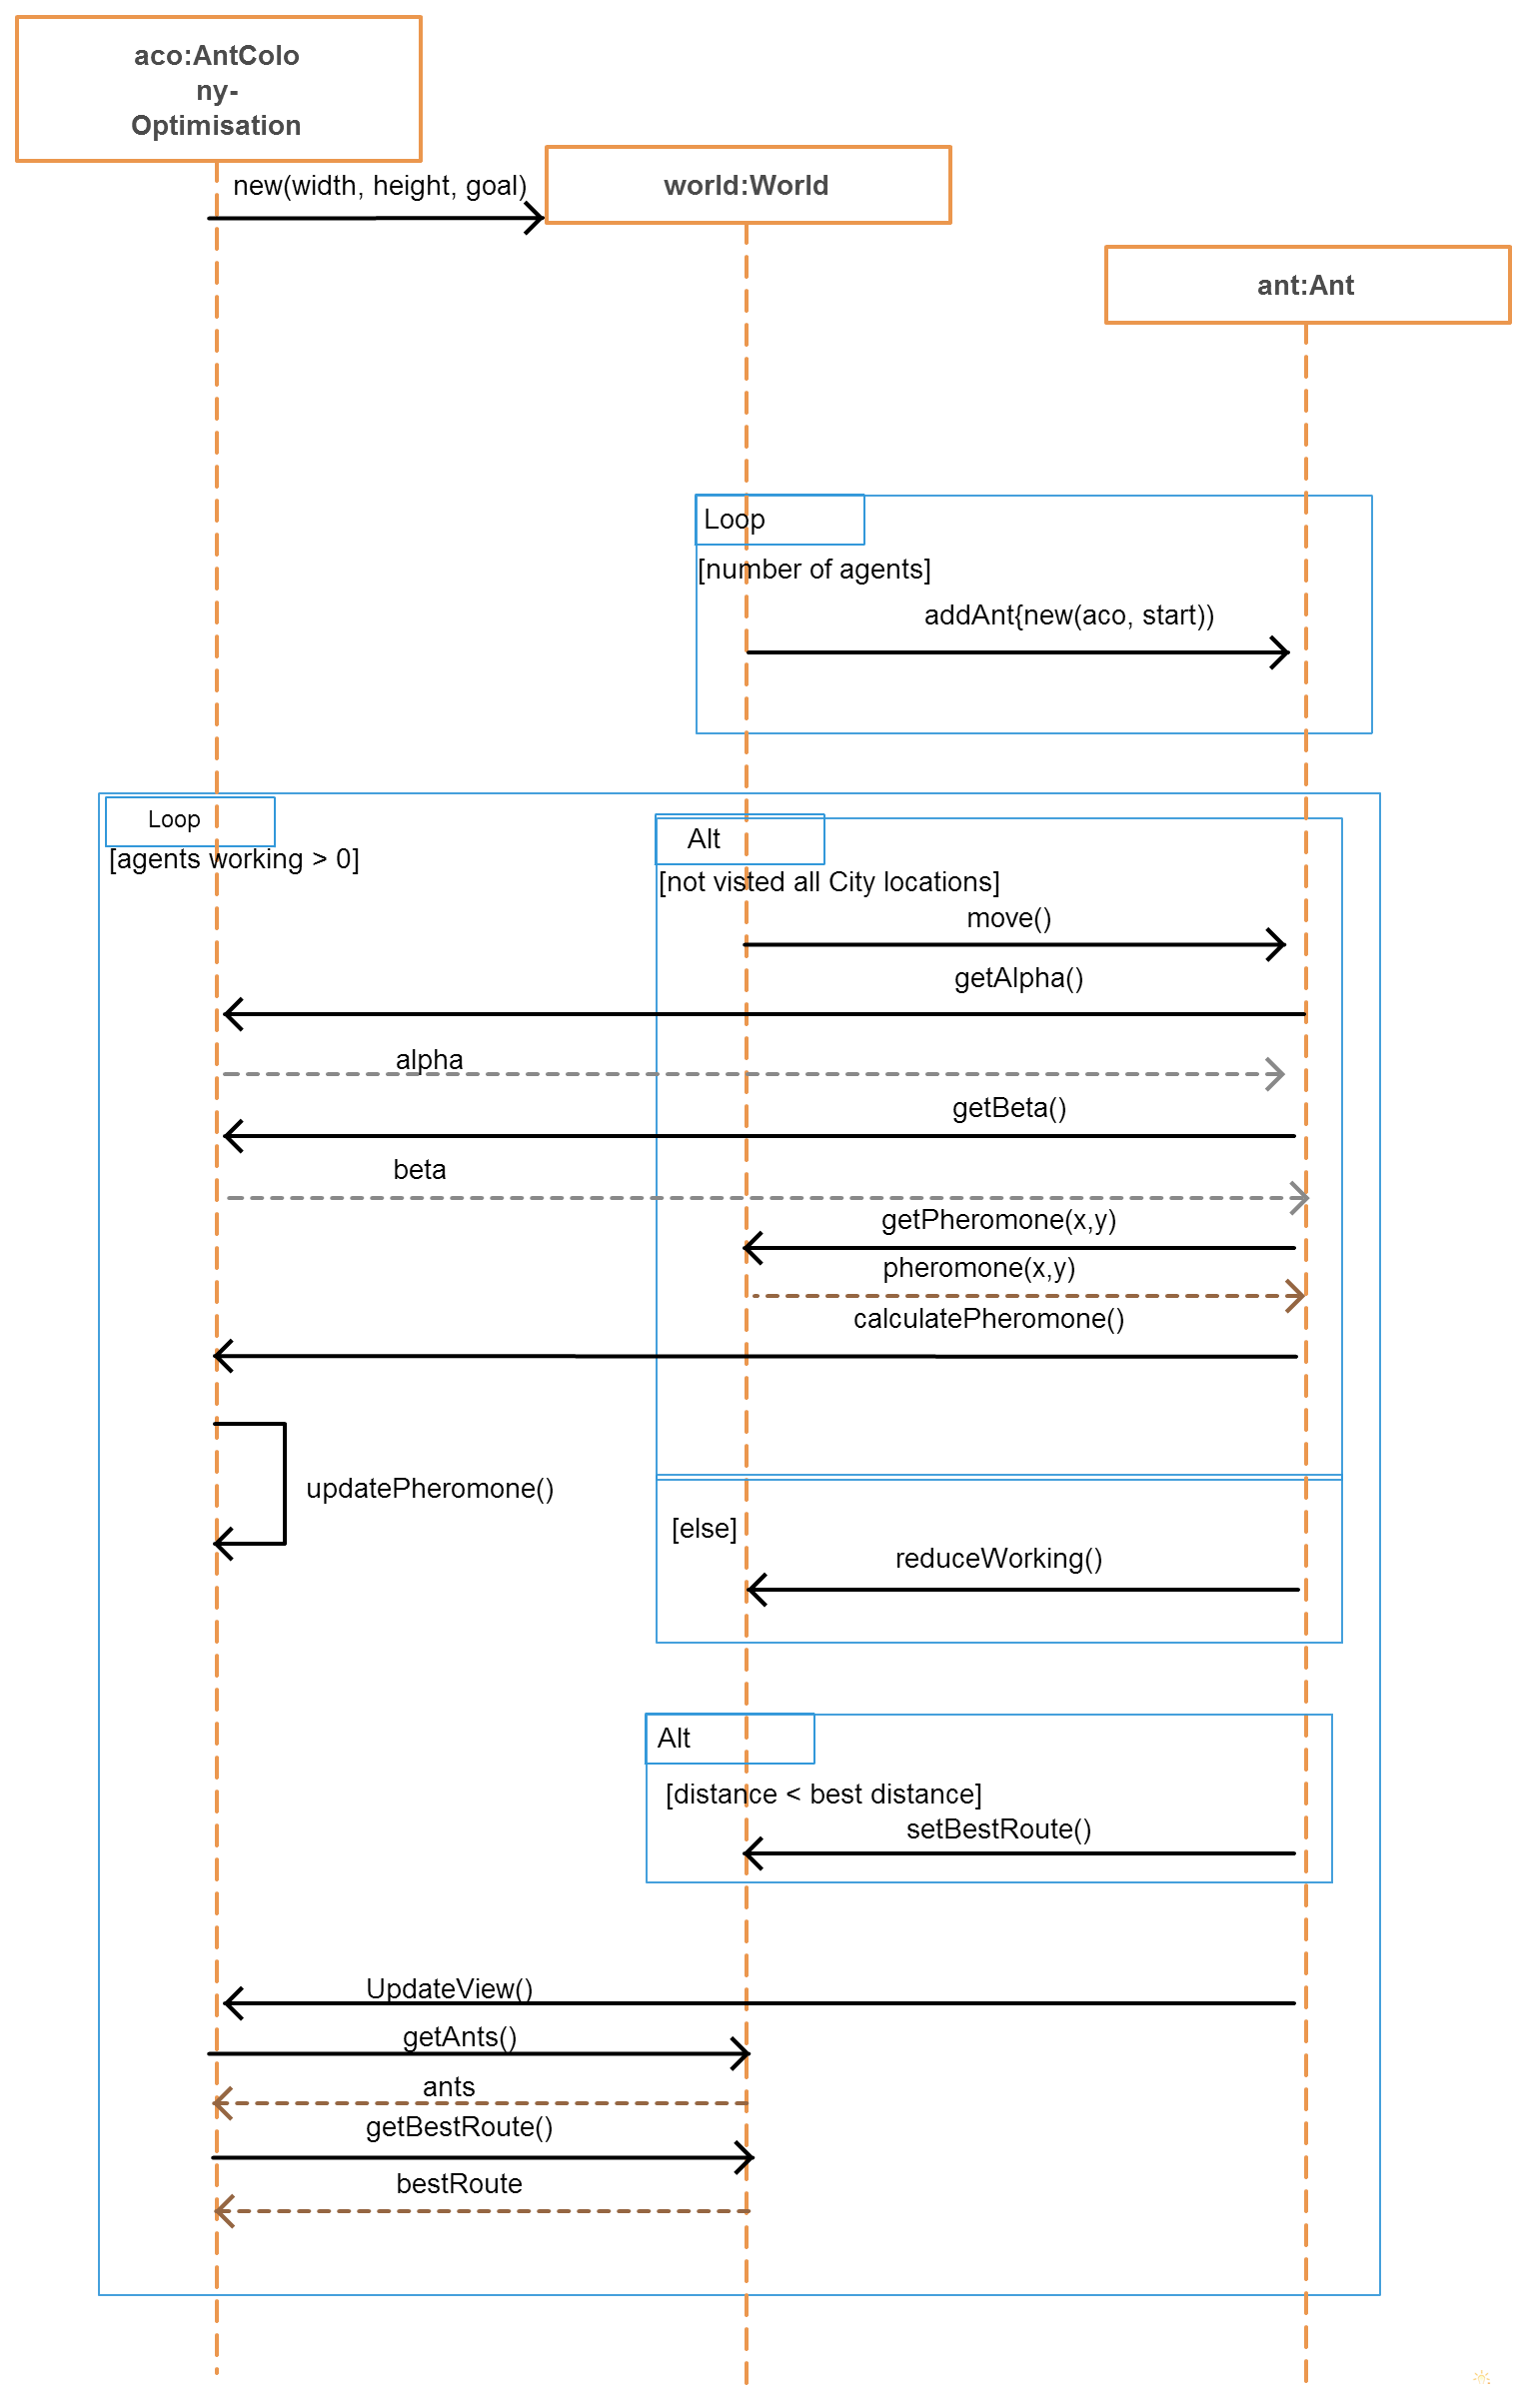
\includegraphics[scale=0.27]{Images/chapter4/sequence}
\caption[Overall Sequence Diagram]{Overview of system interactions based on Algorithm \ref{aco:pseudo2}}
\label{fig:overSeq}
\end{figure}

The sequence diagram described in figure \ref{fig:overSeq} demonstrates at a high level how the algorithm executes. This differs slightly from the initial design (figure \ref{fig:seq}) in order to correctly model the change of problem representation.

\subsection{Formulae}

\subsubsection{Probability}

The probability function is defined in section \ref{sssec:probfuncsssec} appendix B. The design for this algorithm remains unchanged form the pseudo code represented in algorithm \ref{aco:pseudo:probfunc}. The result of this algorithm is in fact, the probability associated with the agent moving to a specific location.

\subsubsection{Pheromone}

The probability function is defined in section \ref{sssec:pherodepo} appendix B. The design for the probability algorithm remains unchanged form the pseudo code represented in algorithm \ref{aco:pseudo:pherofunc}. This is the function that models the pheromone deposit and decay operations.

\subsection{Elitist Ants}

The Elitist Ant algorithm was not initially planned as a feature provided by this application. The author decided that sufficient time was available to produce a brief design for the Elitist ant algorithm extension to allow for a smooth implementation of such design.

\subsubsection{Overview}

The general premise for this Elitist Ant algorithm is defined in section \ref{eliteymcneaty}. The probability function will remain the same as defined in algorithm \ref{aco:pseudo2} whereas the general behaviour of the system and the pheromone deposit function will differ slightly to that of the Basic Ant algorithm. The general system interactions will be the same as shown in figure \ref{fig:overSeq}.


\begin{algorithm}[H]
\caption[Eltist Ant System Pseudo-code]{Pseudo-code for Elitist Ant System implementation}
\label{aco:pseudoEAS}
\begin{algorithmic}[1]
\State Initialise AntColonyOptimisation with defined parameters
\If{$!parameters\ are\ legal$}
\State Dispaly error message to user
\State $return$
\EndIf
\State Initialise World with algorithm parameters
\State Initialise $Nodes$ and graph
\State Initialise \textit{pheromone} values
\State Initialise $Agents$
\While {$!all\ agents\ finished$} 
\ForAll{Agents}
\While{!visited\ all\ $City$\ locations}
\State Calculate next move using probabilistic function 
\State Add location to Agent's memory
\State Update pheromone
\State Update the View
\EndWhile 
\If{total\ stored $Elite Ants\ <$ total\ defined $Elite Ants$}
\State add this ant to elite ants
\Else 
\ForAll{$Elite Ants$}
\State find\ the\ $Elite Ant$ with\ the\ worst\ route
\If{worst\ $Elite Ant$ route is worse than this $Ant$ route}
\State replace\ worst\ $Elite Ant$\ with\ this\ $ant$ 
\EndIf
\State \textbf{end if} 
\EndFor 
\State \textbf{end for}
\EndIf 
\State \textbf{end if}
\State \textbf{end while}
\EndFor 
\State \textbf{end for}
\EndWhile 
\State \textbf{end while}

\If{$\textit{local best solution} < \textit{global best solution}$}
\State $global best = local\ best\ solution$
\EndIf
\State \textbf{end if}
\State \textbf{end while}
\State output \textbf{global best} solution
\end{algorithmic}
\end{algorithm}
%6306 to this point
The difference between aglorithms \ref{aco:pseudoEAS} and \ref{aco:pseudo2} is the manipulation of EliteAnts which is defined in lines 16 to 25. These lines enable the algorithm to constantly ensure that only the best (Elite) $x$ number of ants are stored across iterations to ensure than these pheromone is deposited on the best paths. In order to do this, every time an ant has completed certain checks are made to see if this ant is eligible to become one of the $x$ elite ants. An ant is deemed eligible if the current elite ant collection is not fully populated or if this ant has a better route than the worst performing elite ant. If the later of these two conditions is met then the worst performing elite ant is then swapped with the current ant. This difference can also be observed in figure \ref{fig:overallFlowEAS} which gives an even more abstract overview of the Elitist Ant System.

\clearpage
\begin{sidewaysfigure}
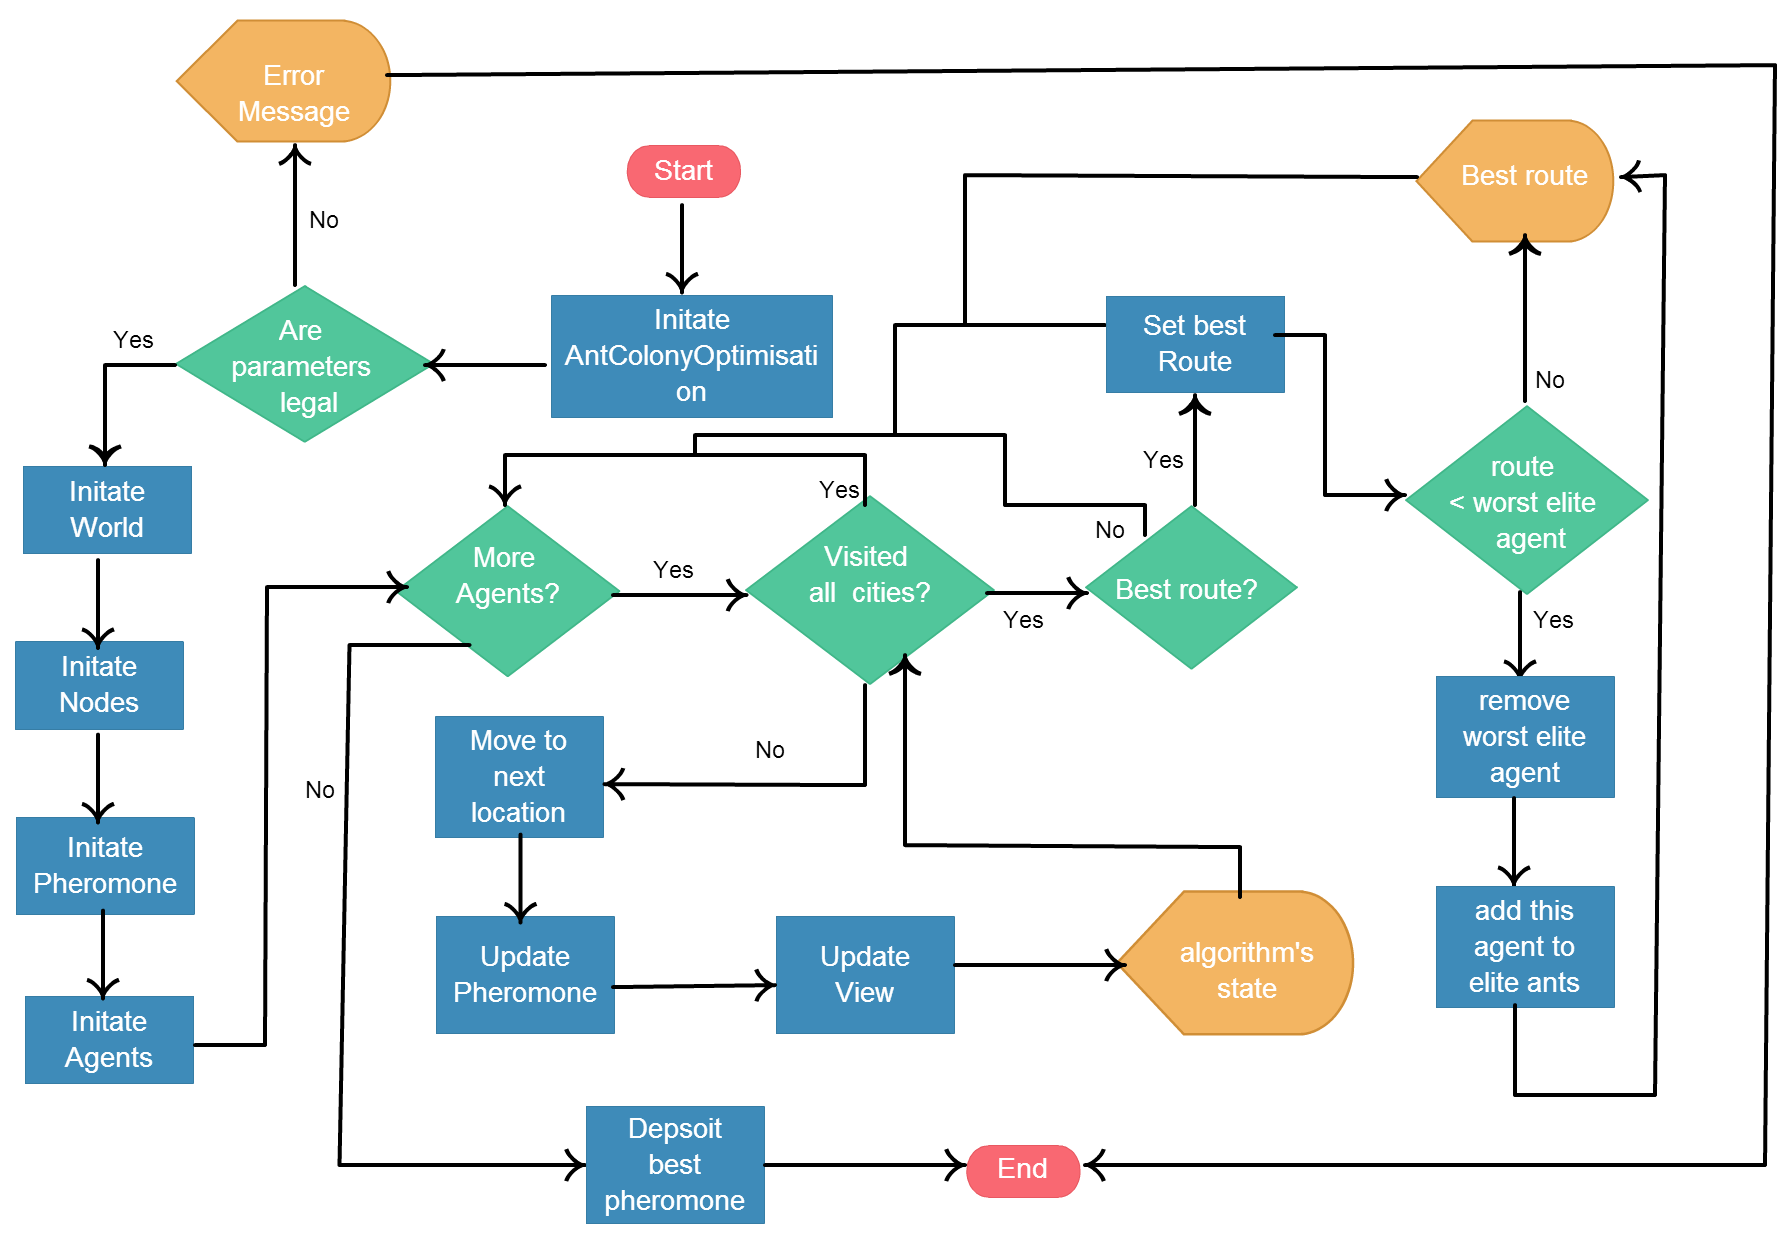
\includegraphics[scale=0.38]{Images/chapter4/eliteAntFlow}
\caption[Elitist Ant System Flow Diagram]{Flow diagram representing algorithm \ref{aco:pseudoEAS}}
\label{fig:overallFlowEAS}
\end{sidewaysfigure}
\clearpage

\subsubsection{Depositing Best Pheromone}

As described in section \ref{eliteymcneaty}, the Elitist Ant System has a slightly different pheromone function to that of the one described in section \ref{sssec:pherodepo} for the Basic Ant system. This modified pheromone function is mostly the same as in the Basic Ant System however, the elite routes must be factored in.

\begin{algorithm}[H]
\caption[Elite Ant System Pseudo-code Pheromone Function]{Elitist Ant System pheromone function pseudo-code}
\label{aco:pseudoEASphero}
\begin{algorithmic}[1]

\State define the $e$ value $=$ $e \times $ \#\ of\ $cities$
\ForAll {stored\ $EliteAnts$}
\State initialise index $i = 0$
\State $currentBest = EliteAnt\ path$ 
\ForAll {$Cities$ along $currentBest$}
\State get the $City\ index$ at $currentBest[i]$
\If{$i + 1 < currentBest\ size$}
\State get the $City index$ at $currentBest[i + 1]$
\State add $e$ amount\ of $new\ pheromone$\ to\ $pheromoneEdge[i][i + 1]$
\EndIf 
\State \textbf{end if}

\State $i++$
\EndFor 
\State \textbf{end for}
\EndFor
\State \textbf{end for}

\end{algorithmic}
\end{algorithm}

Algorithm \ref{aco:pseudoEASphero} demonstrates how the current elite ants are factored into the pheromone function. In general, this will enable the population of agents to converge towards a solution at a faster rate than the Basic Ant System as the increased amount of pheromone on edges used in the current best paths will be greater thus, ants will have a greater probability of traversing such edges.

\subsection{Algorithm Rendering}

Design and development of the algorithm responsible for visualising the Ant Colony algorithm's current state  is one of the more important algorithms in the application as the visualisation process is key to the projects success.

\begin{algorithm}[H]
\caption[Algorithm Visualisation Pseudo-code]{Pseudo-code for rendering of the algorithms execution}
\label{aco:renderPesudo}
\begin{algorithmic}[1]

\State retrieve latest version of the model
\If{model $!null$}
\ForAll{$Cities$ in $model.getWorld().getCities()$}
\State $drawOval(City.X, City.Y, width, height)$

\If{algorithm $!finished$}
\For{$City$}
\ForAll{$Cities$}
\State set opacity based on pheromone value at $edge[city.index][cities.index]$
\State draw a line from $City_{xy}$ to every element in $Cities_{xy}$
\EndFor 
\State \textbf{end for}
\EndFor 
\State \textbf{end for}
\EndIf
\State \textbf{end if}
\EndFor
\State \textbf{end for}
\ForAll{$agents$}
\ForAll{$cities$}
\If{$agent\ location == City.index$}
\State draw agent at $City.x, City.Y$
\State $break$
\EndIf
\State \textbf{end if}
\EndFor
\State \textbf{end for}
\EndFor
\State \textbf{end for}
\If{$best distance > 0$}
\State $best\ route = model.getBestRoute()$
\For{$i = 0$ untill $i <$ $best\ route.size()$}
\If{$i + 1 < \ best\ route.size()$}
\State set colour as red
\State $drawLine(Cities[i].x, cities[i].y, cities[i + 1].x, cities[i + 1].y)$
\EndIf
\State \textbf{end if}
\EndFor
\State \textbf{end for}
\EndIf
\State \textbf{end if}
\EndIf
\State \textbf{end if}

\end{algorithmic}
\end{algorithm}
%6834 untill here

The pseudo code represented in algorithm \ref{acorenderPesudo} defines the design of the general concept used to visualise the underlying algorithm. The author acknowledges that this is not the most efficient or elegant design and this is used an implementation starting point and is by no means a concrete design. Lines 3 to 13 are used to represent the graph visualisation. Drawing a line from every City to every other City will simulate a fully connected graph of cities to the user. The opacity of these lines will be be directly related to the pheromone concentration for the corresponding edge. Lines 22 to 30 show way in which the current best path will be rendered to the user. The author has designed this so that multiple pairs of lines are drawn which will ultimately form one continuous line representing the best path. Each line will have a start and end location, the end location of each line will become the starting location of the next line. This is done by iterating through the pairs of the cities in the best route until there is no longer a valid pair of locations to draw a line between. Once this point is reached the line is complete.